\documentclass[12pt,a4paper]{article}
\usepackage[utf8]{inputenc}%Para Tildes y ñ%
\usepackage[spanish]{babel}
\usepackage{amsmath}
\usepackage{amsfonts}
\usepackage{amssymb}
\usepackage{siunitx}
\usepackage{adjustbox}
%\usepackage{minted}
\usepackage[american]{circuitikz}
\usepackage{tikz}
\usepackage{graphicx} 
\usepackage{pdfpages} %para importar paginas de un pdf 
\usepackage{booktabs}
\usepackage[bookmarks = true, colorlinks=true, linkcolor = black, citecolor = green, menucolor = black, urlcolor = black]{hyperref} 
\usepackage[left=2cm,right=2cm,top=2cm,bottom=2cm]{geometry} 
\usepackage{multirow}
\addto\captionsspanish{\renewcommand{\listtablename}{Índice de tablas}}		% Cambiar nombre a lista de tablas   
\addto\captionsspanish{\renewcommand{\tablename}{Tabla}}					% Cambiar nombre a tablas
\usepackage{float}		% Para ubicar las tablas y figuras justo después del texto
\usepackage{pdfpages}
\usepackage{enumerate}%listas y viñetas
\author{Estudiantes:\\ Kevin Campos Campos\\ Josué Salmerón Córdoba  \\{\small Grupo 1}\\ Profesor:  Marco Villalta  \vspace*{3.0in}}
\title{Universidad de Costa Rica\\{\small Facultad de Ingeniería\\Escuela de Ingeniería Eléctrica\\IE0624 – Laboratorio II\\III ciclo 2023\\\vspace*{0.55in}}\\ Título: GPIOs, Timers y FSM  \vspace*{1.35in}}
%\date{fecha de entrega} 

\begin{document} 

\maketitle  
\thispagestyle{empty}%%no numerar la portada
\renewcommand{\thepage}{\roman{page}}
\newpage
\tableofcontents
\newpage
\listoffigures 
\newpage
\listoftables  
\newpage
%%%%%%%%%%  
\renewcommand{\thepage}{\arabic{page}} 
\setcounter{page}{1}
\begin{center}
\section{Resumen}
En el presente trabajo, se presenta la simulación de una lavadora automática por medio de interrupciones, se definen 3 botones que se encargan de fijar la carga de ropa/artículo que se necesita limpieza, una vez hecho esto la lavadora inicia su labor por medio de un temporizador representado por dos displays de 7S, e indicando por medio de LEDs la carga asignada y el estado de lavado. El uso de interrupciones y una máquina de estados permitió realizar todo lo anterior, es decir, la lavadora funciona correctamente apenas reconoce la carga dada y muestra correctamente todos los pasos, excepto el botón de pausa, que por razones de tiempo no fue posible crearlo ya que no sobraron pines para su diseño, no obstante es un diseño que garantiza el funcionamiento apropiado de una lavadora automática.
\end{center}

%\textbf{\textit{Palabras clave}} \\

%palabras,clave,separadas, por,coma (solo en el reporte)
   
\newpage  


%\section{Objetivos}
\subsection{Objetivos General}
\begin{itemize}
\item obj gral. 

\end{itemize}

\subsection{Objetivos Específicos}
\begin{itemize}
\item objetivo 1
\item objetivo 2  

\end{itemize} 
\newpage
\section{Nota teórica}
En esta sección se muestran las descripciones generales de todos los componentes usados para construir el circuito solicitado.
\subsection*{Microcontrolador ATTiny4313}
El ATtiny2313A/4313 es un microcontrolador CMOS de 8 bits de bajo consumo basado en el AVR mejorado.
Arquitectura RISC. Al ejecutar poderosas instrucciones en un solo ciclo de reloj, el ATtiny2313A/4313 logra rendimientos cercanos a 1 MIPS por MHz, lo que permite al sistema diseñador para optimizar el consumo de energía frente a la velocidad de procesamiento \cite{web}. Por lo que se requiere estudiar el diagrama de pines mostrado en la figura \ref{fig1}
\begin{figure}[H]
\centering
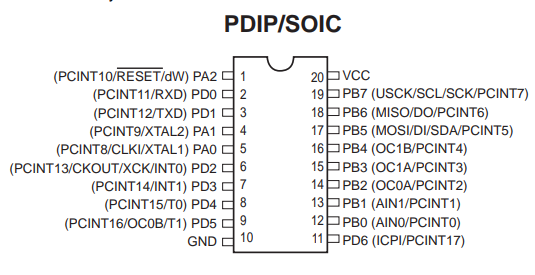
\includegraphics[width=.8\linewidth]{Imagenes/1.png}
 \caption{Pines del ATtiny4313. Tomado de \cite{web}.}
 \label{fig1}
\end{figure}
\subsubsection*{Características generales}
A continuación, se describen las características de cada pin para tener un mejor entendimiento de lo que se puede hacer con cada uno de ellos \cite{web}.
\begin{enumerate}
\item PA2-RESET/dW/PCINT10: RESET: entrada activa en bajo y activada por un 1 el \texttt{RSTDISBL} fuse. El pullup se activa y el controlador de salida y la entrada digital se desactivan cuando se usa el pin de RESET. \texttt{dW}: Cuando el fusible debugWIRE Enable (DWEN) está programado y los bits de bloqueo están sin programar, se activa el sistema debugWIRE dentro del dispositivo de destino. El pin RESET del puerto está configurado como un pin de I/O bidireccional de cable Y (drenaje abierto) con pull-up habilitado y se convierte en la puerta de enlace de comunicación entre el objetivo y el emulador. Sirve como I/O y tiene la opción de RESET. Solo que debe ponersele un 0 para que funcione como I/O. Tiene una resistencia interna de pull up. \texttt{PCINT10}: Fuente de interrupción de cambio de pin. El pin PA2 sirve como una fuente de interrupción externa.

\item PD0-RXD/PCINT11. \texttt{RXD}: UART receptor de datos. \texttt{PCINT11}: El pin PD0 sirve como fuente de interrupción externa.

\item PD1-TXD/PCINT12. \texttt{TXD}: UART transmisor de datos. \texttt{PCINT12}: El pin PD0 sirve como fuente de interrupción externa.

\item PA1-XTAL2/PCINT9. \texttt{XTAL2}: chip de reloj oscilador. Se utiliza como pin de reloj para todas las fuentes de reloj de chip excepto oscilador RC interno calibrable y reloj externo. Cuando se utiliza como pin de reloj, el pin no se puede utilizar como pin de I/O. Cuando se utiliza un oscilador RC interno calibrable o un reloj externo como en las fuentes de reloj del chip, PA1 sirve como un pin de I/O normal. Este pin sirve como fuente de interrupción externa.
\item PA0-\texttt{XTAL1/CLKI/PCINT8}. \texttt{XTAL1}: oscilador de reloj de chip. Se utiliza para todas las fuentes de reloj de chip excepto oscilador RC interno calibrable. Cuando se usa como pin de reloj, el pin no se puede usar como pin de I/O. Cuando se utiliza un oscilador RC interno calibrable como fuente de reloj de chip, PA0 sirve como pin de I/O. Este pin sirve como fuente de interrupción externa.
\item PD2-INT0/XCK/CKOUT/PCINT13. \texttt{INTO}: este pin sirve como fuente de interrupción externa para el MCU. \texttt{XCK}: USART Reloj de transferencia utilizado sólo en el modo de transferencia síncrona.\texttt{CKOUT}: reloj sistema de salida.
\item PD3-INT1/PCINT14. Ambas descripciones representan la misma equivalencia, ya que su objetivo final es que el pin PD3 sirve como fuente de interrupción externa.
\item PD4-TO/PCINT15. \texttt{TO}: timer/counter0 la entrada del reloj contador externo se habilita configurando (uno) los bits CS02 y CS01 en el registro de control del timer/counter0 (TCCR0).\texttt{PCINT15}: este pin sirve como fuente de interrupción externa.
\item PD5-OC0B/T1/PCINT16.\texttt{OC0B}:  Output Compare Match B. \texttt{T1}: La entrada del contador externo se habilita configurando (uno) los bits CS02
y CS01 en el registro de control del timer1/counter1 (TCCR1) \texttt{PCINT16}: este pin sirve como fuente de interrupción externa.
\item GND: nodo de tierra.
\item PD6-ICPI/PCINT17.\texttt{ICPI}: entrada de captura. Este pin puede actuar como un pin de captura de entrada para el timer/counter1. \texttt{PCINT17}: este pin sirve como fuente de interrupción externa.
\item PB0-AIN0/PCINT0. \texttt{AIN0}: es un comparador análogo de entrada positiva. Configure el pin del puerto como entrada con el pull-up interno apagado para evitar que la función del puerto digital interfiera con la función del comparador analógico \texttt{PCINT0}: este pin sirve como fuente de interrupción externa.
\item PB1-AIN1/PCINT1. \texttt{AIN1}: es un comparador análogo de entrada negativa. \texttt{PCINT1}: este pin sirve como fuente de interrupción externa.
\item PB2-OC0A/PCINT2.Output Compare Match A output. \texttt{OC0A}: el pin PB2 puede servir como salida externa para comparación de salida de timer/counter0 A. El pin debe configurarse como salida (configurando DDB2 igual 1) y cumplir esta función. \texttt{PCINT2}: este pin sirve como fuente de interrupción externa.
\item PB3-OC1A/PCINT3. \texttt{OC1A}:Output Compare Match A output. El pin PB3 puede servir como salida externa para comparación de salida de timer/counter1 A. El pin debe configurarse como salida (configurando DDB3 igual 1) y cumplir esta función. \texttt{PCINT3}: este pin sirve como fuente de interrupción externa.
\item PB4-OC1B/PCINT4. \texttt{OC1B}: Output Compare Match B output. Se puede configurar DDB4 igual a 1 para activar esta función. \texttt{PCINT4}: este pin sirve como fuente de interrupción externa.
\item PB5-DI/SDA/PCINT5.\texttt{DI}: Entrada de datos de interfaz serie universal en modo de tres cables. El modo de tres cables no anula las funciones normales del puerto, por lo que el pin debe configurarse como entrada.\texttt{SDA}: modo serial interfaz de datos de dos cables.\texttt{PCINT5}: este pin sirve como fuente de interrupción externa.
\item PB6-DO/PCINT6. \texttt{DO}: Salida de datos de interfaz serie universal en modo de tres cables. Modo de tres cables de salida de datos anula el valor de PORTB6 y se dirige al puerto cuando el bit de dirección de datos DDB6 es uno. Sin embargo, el bit PORTB6 aún controla el pull-up, lo que permite el pull-up si se ingresa la dirección y PORTB6 en 1. \texttt{PCINT6}: este pin sirve como fuente de interrupción externa.
\item PB7-USCK/SCL/PCINT7. \texttt{USCK}: interfaz serial de reloj modo de 3 cables. \texttt{SCL}: reloj serial para USI modo de dos cables. \texttt{PCINT7}: este pin sirve como fuente de interrupción externa.
\item VCC: fuente de alimentación.
\end{enumerate}
En la figura \ref{fig2} se muestra el diagrama de bloques de este microcontrolador.
\begin{figure}[H]
\centering
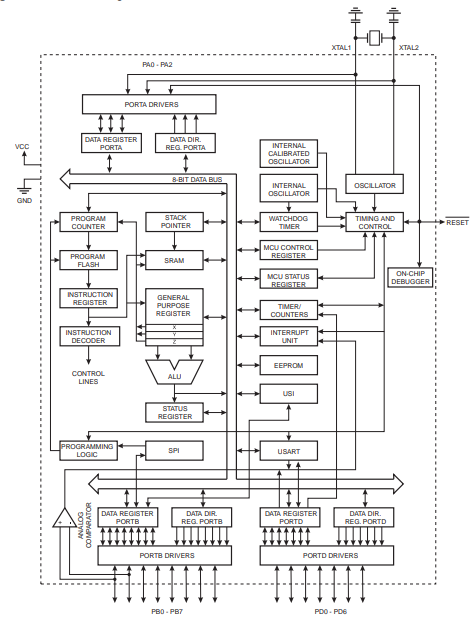
\includegraphics[width=.7\linewidth]{Imagenes/2.png}
 \caption{Diagrama de bloques del ATtiny4313. Tomado de \cite{web}.}
 \label{fig2}
\end{figure}
Otro detalle importante es considerar los valores máximos con los que se puede trabajar el ATtiny4313.
\begin{figure}[H]
\centering
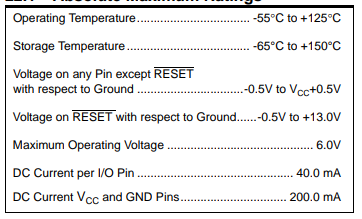
\includegraphics[width=.5\linewidth]{Imagenes/3.png}
 \caption{Diagrama de bloques del ATtiny4313. Tomado de \cite{web}.}
 \label{fig3}
\end{figure}

\subsection*{Periféricos}
La descripción de los registros e instrucciones utilizados son los siguientes:
\begin{itemize}
    \item \textbf{DDRxn}: Registro de dirección de datos. Encargado de determinar si los pines van a trabajar como entradas (0) o como salidas (1). El registro de dirección de datos se observa en la siguiente imagen:
    \begin{figure}[H]
        \centering
        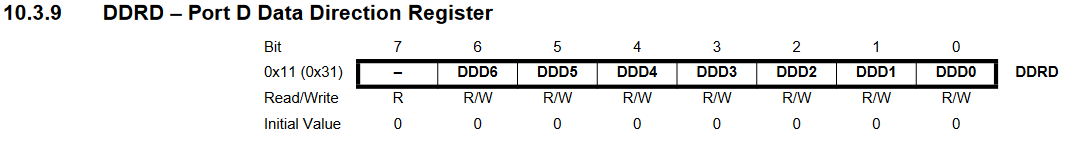
\includegraphics[width=.9\linewidth]{Imagenes/DirectionD.png}
        \caption{Registro de dirección de datos. Tomado de \cite{web}.}
        \label{fig4}
    \end{figure}
    
	\item \textbf{PORTxn}: Registro de datos. Permite establecer los pines con un estado inicial, ya sea en alto o en bajo, esto para el uso de señales digitales.
    \begin{figure}[H]
        \centering
        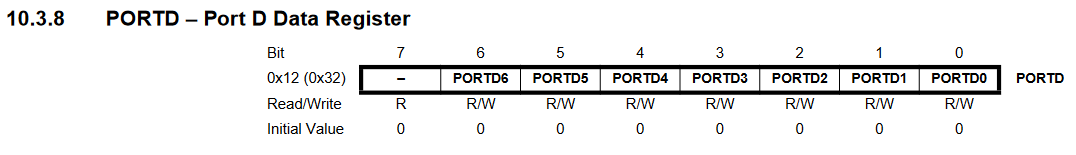
\includegraphics[width=.9\linewidth]{Imagenes/DataD.png}
        \caption{Registro de datos. Tomado de \cite{web}.}
        \label{fig5}
    \end{figure}

    \item \textbf{GIMSK}: (General Interrupt Mask Register). Registro encargado de habilitar y deshabilitar interrupciones. Cuando se desea leer interrupciones es necesario configurar este registro.
    \begin{figure}[H]
        \centering
        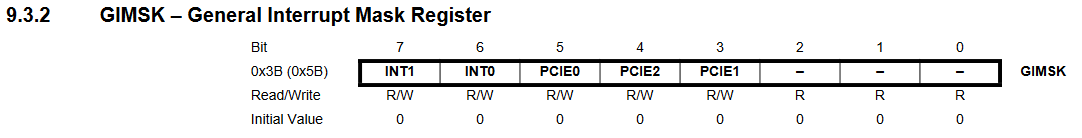
\includegraphics[width=.9\linewidth]{Imagenes/GIMSK.png}
        \caption{Configuración del registro GIMSK. Tomado de \cite{web}.}
        \label{fig6}
    \end{figure}

    \item \textbf{PCMSKn}: Usado para habilitar o deshabilitar ciertos pines para que trabajen como pines de interrupción.
    \begin{figure}[H]
        \centering
        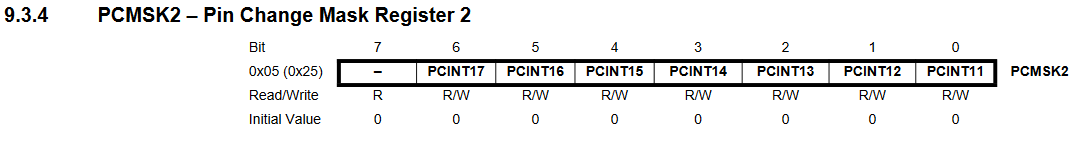
\includegraphics[width=.9\linewidth]{Imagenes/PCMSK.png}
        \caption{Registro habilitación de interrupciones. Tomado de \cite{web}.}
        \label{fig7}
    \end{figure}

    \item \textbf{TCCR0x}: Este es el registro de control para el contador 0 (x puede ser A o B), además, permite establecer el prescaler y modos de comparación. Hay dos registros de control para el contador 0, ya sea el A o el B.
    \begin{figure}[H]
        \centering
        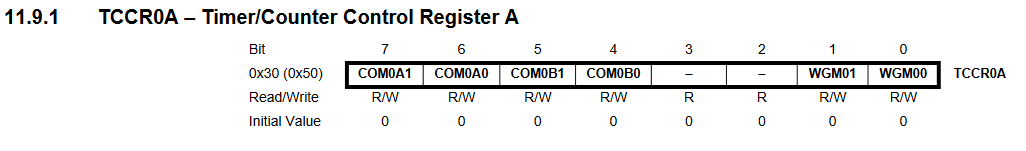
\includegraphics[width=.9\linewidth]{Imagenes/TCCR0A.png}
        \caption{Registro de control de Timer/Counter. Tomado de \cite{web}.}
        \label{fig8}
    \end{figure}

    \item \textbf{OCR0A}: Registro que guarda el valor de comparación. Cuando el valor de OCR0A es igual al de TCNT0 la señal del comparador se pone en alto.
    \begin{figure}[H]
        \centering
        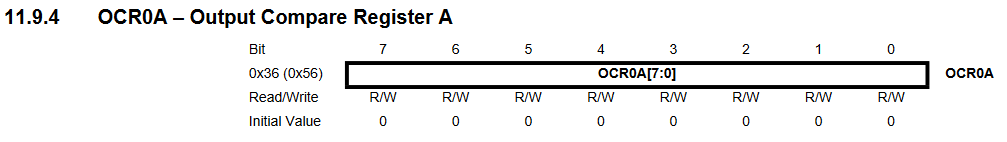
\includegraphics[width=.9\linewidth]{Imagenes/OCR0A.png}
        \caption{Registro de comparación de salida A. Tomado de \cite{web}.}
        \label{fig9}
    \end{figure}
    
\end{itemize}

\subsection*{Componentes electrónicos complementarios}
\subsubsection*{Decodificador BCD y display de 7 segmentos}
BCD (Decimal Codificado en Binario) es un código que representa valores decimales en formato binario, para ello forma grupos de 4 bits para representar cada valor del 0 al 9. El 9 es el valor máximo que se puede representar en un dígito decimal \cite{web2}. Lo anterior justifica el hecho de usar dos display de 7 segmentos, al tener 2 de estos componentes es necesario usar dos convertidores ya que se necesita optimizar la cantidad de pines del MCU \texttt{ATtiny4313}.
    \begin{figure}[H]
        \centering
        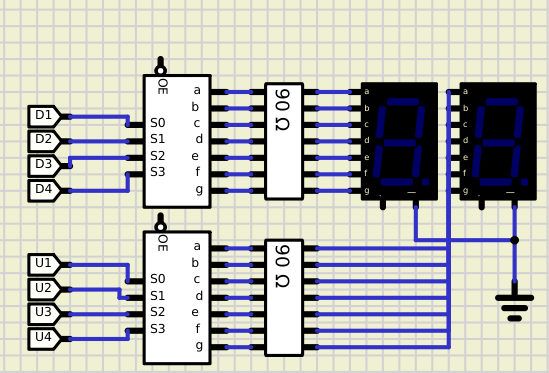
\includegraphics[width=.5\linewidth]{Imagenes/4.png}
        \caption{Conexión de los displays con el ATtiny4313. Tomado de \cite{web}.}
        \label{fig10}
    \end{figure}
\subsubsection*{Switches}
Los botones son elementos importantes para poder activar las interrupciones, no obstante, hay que tener en cuenta el efecto rebote para evitar las lecturas falsas en el circuito.
    \begin{figure}[H]
        \centering
        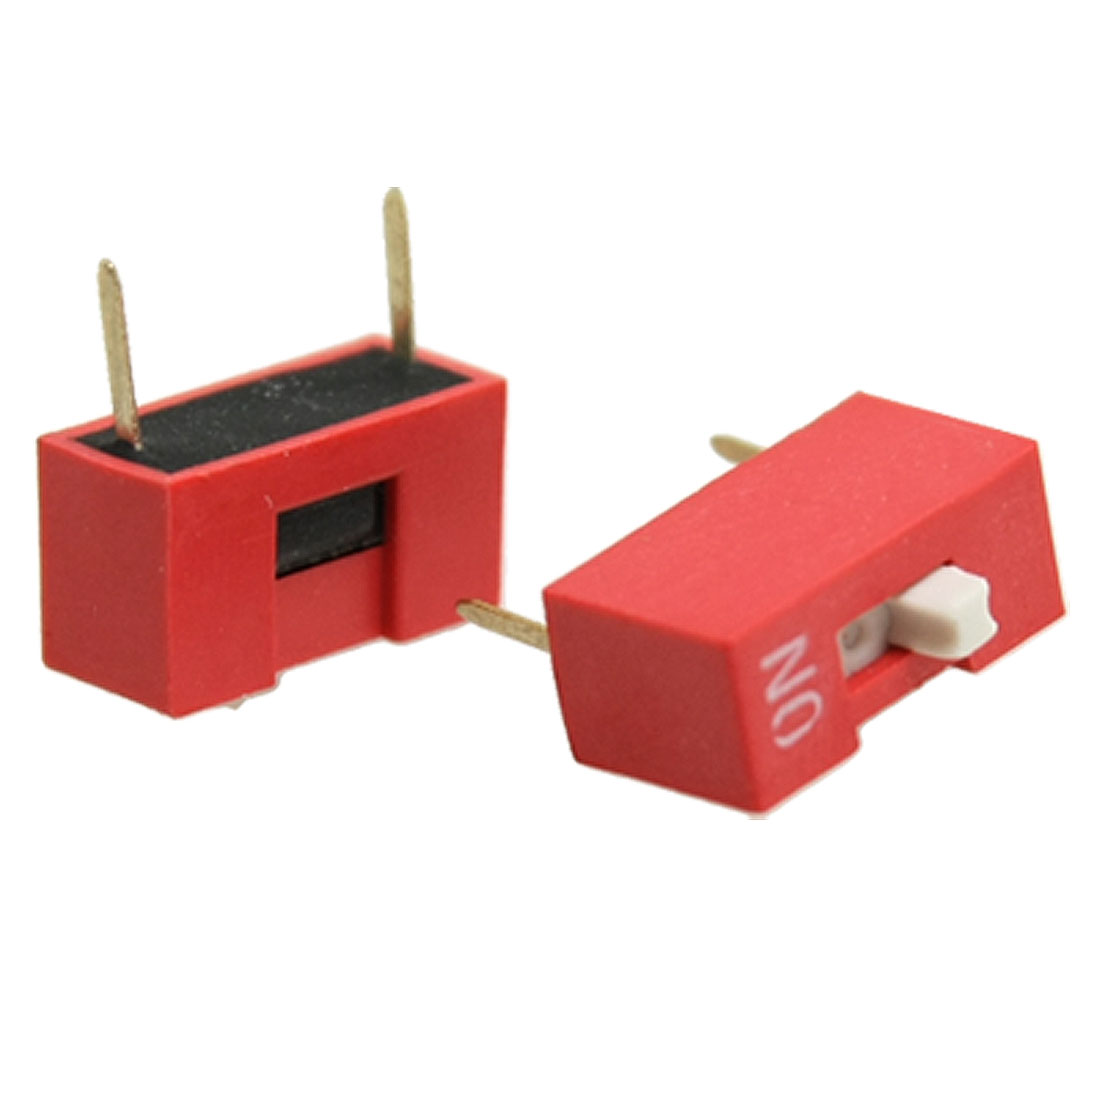
\includegraphics[width=.3\linewidth]{Imagenes/switch.jpeg}
        \caption{Botones. Tomado de \cite{web3}.}
        \label{boton}
    \end{figure}

\subsubsection*{LEDs}
Los Leds se encargarán de mostrar los estados de la lavadora, y para estos hay que ponerles una resistencia adecuada para no afectar este tipo de señales. Por este motivo, se procuro operar bajo tensiones eléctricas menores a \SI{2.4}{\volt}.
    \begin{figure}[H]
        \centering
        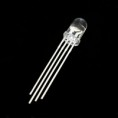
\includegraphics[width=.3\linewidth]{Imagenes/LED.jpg}
        \caption{LEDs. Tomado de \cite{web3}.}
        \label{LED}
    \end{figure}
    
\subsubsection*{demultiplexor}
Es un decodificador/demultiplexor dual 1 de 4 de alta velocidad. El dispositivo tiene dos decodificadores independientes, cada uno de los cuales acepta dos entradas y proporcionando cuatro salidas LOW activas mutuamente excluyentes \cite{web3}. Se adaptó este componente para configurar la salida de los LEDs y así poderlos conectar al MCU.
    \begin{figure}[H]
        \centering
        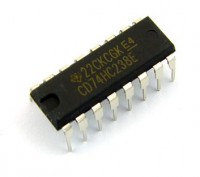
\includegraphics[width=.3\linewidth]{Imagenes/demux.jpg}
        \caption{Demultiplexor. Tomado de \cite{web3}.}
        \label{demux}
    \end{figure}
    
\subsection*{Lista de componentes}
En la tabla \ref{table_2} resume el equipo electrónico a usar para este laboratorio.\par \textbf{Nota:} Se encontró un kit donde vienen todas las magnitudes buscadas, \SI{100}{\ohm}, \SI{100}{\kilo\ohm}, \SI{10}{\kilo\ohm}
\begin{table}[H]
\caption{Lista de equipos}
\label{table_2}
\begin{center}
\begin{tabular}{r|cc}
\hline
\textbf{Componente}&\textbf{Cantidad}&\textbf{Precio}\\
 \hline
ATtiny4313 &1  & 1.83\$ \\ \hline 
LED 7 segmentos& 2 &1.30\$ \\ \hline 
Resistencias & 1 &9.95\$ \\ \hline

Capacitores \SI{100}{\nano\farad}& 4 & 0.76\$ \\ \hline
Switches & 4 & 2.6\$ \\ \hline
LEDs& 7 & 3.85\$ \\ \hline
Demultiplexor& 1 & 2.35\$ \\ \hline
Convertidores Bcd-7S& 2 &2.60\$ \\ \hline
 \textbf{Total}& & 25.24\$ \\
 \hline
\end{tabular}
\end{center}
\end{table}

\subsection*{Diseño del circuito}

Al tratarse de una lavadora compuesta de máquina de estados, el diseño del circuito se fue realizando por etapas. No obstante, la lógica de la electrónica fue posible armarla con los conocimientos adquiridos del primer laboratorio. El esquemático base para la lavadora automática es el siguiente:
 
\begin{figure}[H]
    \centering


\tikzset{every picture/.style={line width=0.75pt}} %set default line width to 0.75pt        

\begin{tikzpicture}[x=0.75pt,y=0.75pt,yscale=-1,xscale=1]
%uncomment if require: \path (0,715); %set diagram left start at 0, and has height of 715

%Shape: Rectangle [id:dp3736426956156411] 
\draw   (385,175) -- (385,309) -- (317,309) -- (317,175) -- cycle ;
%Shape: Ellipse [id:dp5208816731227319] 
\draw  [fill={rgb, 255:red, 74; green, 144; blue, 226 }  ,fill opacity=1 ] (480.28,182) .. controls (487.66,181.95) and (493.69,187.72) .. (493.74,194.9) .. controls (493.79,202.08) and (487.84,207.94) .. (480.46,208) .. controls (473.07,208.06) and (467.05,202.28) .. (467,195.1) .. controls (466.95,187.92) and (472.9,182.06) .. (480.28,182) -- cycle ;
%Shape: Ellipse [id:dp31358253590072604] 
\draw  [fill={rgb, 255:red, 122; green, 199; blue, 42 }  ,fill opacity=1 ] (480.56,222.62) .. controls (487.94,222.57) and (493.97,228.34) .. (494.02,235.52) .. controls (494.06,242.7) and (488.12,248.57) .. (480.74,248.62) .. controls (473.35,248.68) and (467.33,242.9) .. (467.28,235.72) .. controls (467.23,228.55) and (473.18,222.68) .. (480.56,222.62) -- cycle ;
%Shape: Ellipse [id:dp8142692383830192] 
\draw  [fill={rgb, 255:red, 189; green, 16; blue, 224 }  ,fill opacity=1 ] (480.81,260) .. controls (488.2,259.94) and (494.22,265.72) .. (494.27,272.9) .. controls (494.32,280.08) and (488.37,285.94) .. (480.99,286) .. controls (473.61,286.05) and (467.58,280.28) .. (467.53,273.1) .. controls (467.49,265.92) and (473.43,260.05) .. (480.81,260) -- cycle ;
%Shape: Ellipse [id:dp4276205049596655] 
\draw  [fill={rgb, 255:red, 248; green, 231; blue, 28 }  ,fill opacity=1 ] (481.08,299) .. controls (488.46,298.94) and (494.49,304.72) .. (494.54,311.9) .. controls (494.59,319.08) and (488.64,324.94) .. (481.26,325) .. controls (473.87,325.05) and (467.85,319.28) .. (467.8,312.1) .. controls (467.75,304.92) and (473.7,299.05) .. (481.08,299) -- cycle ;
%Shape: Circle [id:dp40317748688735877] 
\draw  [fill={rgb, 255:red, 4; green, 248; blue, 69 }  ,fill opacity=1 ] (205,233) .. controls (205,224.16) and (212.16,217) .. (221,217) .. controls (229.84,217) and (237,224.16) .. (237,233) .. controls (237,241.84) and (229.84,249) .. (221,249) .. controls (212.16,249) and (205,241.84) .. (205,233) -- cycle ;
%Shape: Circle [id:dp929270239106259] 
\draw  [fill={rgb, 255:red, 80; green, 227; blue, 194 }  ,fill opacity=1 ] (206,279) .. controls (206,270.16) and (213.16,263) .. (222,263) .. controls (230.84,263) and (238,270.16) .. (238,279) .. controls (238,287.84) and (230.84,295) .. (222,295) .. controls (213.16,295) and (206,287.84) .. (206,279) -- cycle ;
%Shape: Circle [id:dp9165194483708052] 
\draw  [fill={rgb, 255:red, 231; green, 142; blue, 60 }  ,fill opacity=1 ] (206,321) .. controls (206,312.16) and (213.16,305) .. (222,305) .. controls (230.84,305) and (238,312.16) .. (238,321) .. controls (238,329.84) and (230.84,337) .. (222,337) .. controls (213.16,337) and (206,329.84) .. (206,321) -- cycle ;
%Shape: Diagonal Stripe [id:dp5302916907355721] 
\draw   (249.63,323.37) -- (201.01,371.99) -- (200.99,178.51) -- (249.62,226.63) -- cycle ;
%Shape: Diagonal Stripe [id:dp8210793156928873] 
\draw   (445.75,195.75) -- (501.75,139.75) -- (504,366) -- (446.87,308.87) -- cycle ;
%Rounded Rect [id:dp3004953074437984] 
\draw   (166,124.2) .. controls (166,117.46) and (171.46,112) .. (178.2,112) -- (222.8,112) .. controls (229.54,112) and (235,117.46) .. (235,124.2) -- (235,160.8) .. controls (235,167.54) and (229.54,173) .. (222.8,173) -- (178.2,173) .. controls (171.46,173) and (166,167.54) .. (166,160.8) -- cycle ;
%Shape: Right Angle [id:dp24099551796063645] 
\draw   (268,138) -- (349,138) -- (349,151) ;
%Straight Lines [id:da7971995572458987] 
\draw    (245,138) -- (268,138) ;
\draw [shift={(242,138)}, rotate = 0] [fill={rgb, 255:red, 0; green, 0; blue, 0 }  ][line width=0.08]  [draw opacity=0] (8.93,-4.29) -- (0,0) -- (8.93,4.29) -- cycle    ;
%Straight Lines [id:da13882289529478786] 
\draw    (177,282) -- (196,282) ;
\draw [shift={(199,282)}, rotate = 180] [fill={rgb, 255:red, 0; green, 0; blue, 0 }  ][line width=0.08]  [draw opacity=0] (8.93,-4.29) -- (0,0) -- (8.93,4.29) -- cycle    ;
%Straight Lines [id:da6747920204662456] 
\draw    (170,326) -- (195,326) ;
\draw [shift={(198,326)}, rotate = 180] [fill={rgb, 255:red, 0; green, 0; blue, 0 }  ][line width=0.08]  [draw opacity=0] (8.93,-4.29) -- (0,0) -- (8.93,4.29) -- cycle    ;
%Straight Lines [id:da9768277231011067] 
\draw    (303,264.06) -- (255,264.94) ;
\draw [shift={(252,265)}, rotate = 358.94] [fill={rgb, 255:red, 0; green, 0; blue, 0 }  ][line width=0.08]  [draw opacity=0] (8.93,-4.29) -- (0,0) -- (8.93,4.29) -- cycle    ;
\draw [shift={(306,264)}, rotate = 178.94] [fill={rgb, 255:red, 0; green, 0; blue, 0 }  ][line width=0.08]  [draw opacity=0] (8.93,-4.29) -- (0,0) -- (8.93,4.29) -- cycle    ;
%Straight Lines [id:da6028101348020392] 
\draw    (349,151) -- (349,167) ;
\draw [shift={(349,170)}, rotate = 270] [fill={rgb, 255:red, 0; green, 0; blue, 0 }  ][line width=0.08]  [draw opacity=0] (8.93,-4.29) -- (0,0) -- (8.93,4.29) -- cycle    ;
%Straight Lines [id:da36652659818902866] 
\draw    (440,252.06) -- (392,252.94) ;
\draw [shift={(389,253)}, rotate = 358.94] [fill={rgb, 255:red, 0; green, 0; blue, 0 }  ][line width=0.08]  [draw opacity=0] (8.93,-4.29) -- (0,0) -- (8.93,4.29) -- cycle    ;
\draw [shift={(443,252)}, rotate = 178.94] [fill={rgb, 255:red, 0; green, 0; blue, 0 }  ][line width=0.08]  [draw opacity=0] (8.93,-4.29) -- (0,0) -- (8.93,4.29) -- cycle    ;
%Straight Lines [id:da7538047830884007] 
\draw    (351,310) -- (351,326) ;
\draw [shift={(351,329)}, rotate = 270] [fill={rgb, 255:red, 0; green, 0; blue, 0 }  ][line width=0.08]  [draw opacity=0] (8.93,-4.29) -- (0,0) -- (8.93,4.29) -- cycle    ;
%Straight Lines [id:da9253882848450912] 
\draw    (509,194) -- (532,194) ;
\draw [shift={(506,194)}, rotate = 0] [fill={rgb, 255:red, 0; green, 0; blue, 0 }  ][line width=0.08]  [draw opacity=0] (8.93,-4.29) -- (0,0) -- (8.93,4.29) -- cycle    ;
%Straight Lines [id:da6111221033767795] 
\draw    (509,230) -- (532,230) ;
\draw [shift={(506,230)}, rotate = 0] [fill={rgb, 255:red, 0; green, 0; blue, 0 }  ][line width=0.08]  [draw opacity=0] (8.93,-4.29) -- (0,0) -- (8.93,4.29) -- cycle    ;
%Straight Lines [id:da34811704409363275] 
\draw    (508,274) -- (531,274) ;
\draw [shift={(505,274)}, rotate = 0] [fill={rgb, 255:red, 0; green, 0; blue, 0 }  ][line width=0.08]  [draw opacity=0] (8.93,-4.29) -- (0,0) -- (8.93,4.29) -- cycle    ;
%Straight Lines [id:da1830384445783324] 
\draw    (510,313) -- (533,313) ;
\draw [shift={(507,313)}, rotate = 0] [fill={rgb, 255:red, 0; green, 0; blue, 0 }  ][line width=0.08]  [draw opacity=0] (8.93,-4.29) -- (0,0) -- (8.93,4.29) -- cycle    ;
%Straight Lines [id:da18201226072077015] 
\draw    (557,201) -- (557,217) ;
\draw [shift={(557,220)}, rotate = 270] [fill={rgb, 255:red, 0; green, 0; blue, 0 }  ][line width=0.08]  [draw opacity=0] (8.93,-4.29) -- (0,0) -- (8.93,4.29) -- cycle    ;
%Straight Lines [id:da6548335593243826] 
\draw    (557,240) -- (557,256) ;
\draw [shift={(557,259)}, rotate = 270] [fill={rgb, 255:red, 0; green, 0; blue, 0 }  ][line width=0.08]  [draw opacity=0] (8.93,-4.29) -- (0,0) -- (8.93,4.29) -- cycle    ;
%Straight Lines [id:da32772831053343854] 
\draw    (558,283) -- (558,299) ;
\draw [shift={(558,302)}, rotate = 270] [fill={rgb, 255:red, 0; green, 0; blue, 0 }  ][line width=0.08]  [draw opacity=0] (8.93,-4.29) -- (0,0) -- (8.93,4.29) -- cycle    ;

% Text Node
\draw (168,129) node [anchor=north west][inner sep=0.75pt]   [align=left] {{\footnotesize ON/STOP}};
% Text Node
\draw (346,180) node [anchor=north west][inner sep=0.75pt]   [align=left] {A\\T\\t\\i\\n\\y};
% Text Node
\draw (135,272) node [anchor=north west][inner sep=0.75pt]   [align=left] {media};
% Text Node
\draw (138,224) node [anchor=north west][inner sep=0.75pt]   [align=left] {baja};
% Text Node
\draw (141,314) node [anchor=north west][inner sep=0.75pt]   [align=left] {alta};
% Text Node
\draw (531,184) node [anchor=north west][inner sep=0.75pt]   [align=left] {Suministro};
% Text Node
\draw (537,220) node [anchor=north west][inner sep=0.75pt]   [align=left] {Lavar};
% Text Node
\draw (536,264) node [anchor=north west][inner sep=0.75pt]   [align=left] {Enjuage};
% Text Node
\draw (535,304) node [anchor=north west][inner sep=0.75pt]   [align=left] {Centrifugar};
\draw (324,355) node[seven segment val=9 dot off box on]{};
\draw (374,355) node[seven segment val=9 dot none box on]{};

\end{tikzpicture}
    \caption{Esquemático general}
    \label{FigWW}
\end{figure}

Del esquemático \ref{FigWW}, es claro notar que el circuito general se compone de varias etapas. Así, es importante saber el uso de las interrupciones para realizar una tarea tan simple como encender o apagar un LED, por ese motivo, hay que consultar la hoja del fabricante del MCU para tener más detalles de los pines para programar la interrupción, además habilitarlos para que sirvan como salida o entrada dependiendo de la conexión hecha previamente. El ejemplo de la figura \ref{fig11},
    \begin{figure}[H]
        \centering
        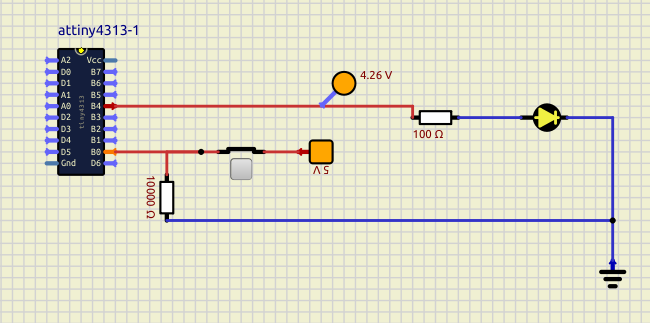
\includegraphics[width=.7\linewidth]{Imagenes/5.1.png}
        \caption{Encendido de un LED.}
        \label{fig11}
    \end{figure}
se muestra que el pin B0, es una entrada para este caso, y esto indica que ocupará habilitar la resistencia de pull-up con el enmáscarado \texttt{GIMSK}. Por su parte, el pin B4 se trata de una salida, entonces basta con hacer uso de \texttt{DDRB=0b00010000}, para que el programa entienda que es una salida. De esa manera, presionando el botón, es posible encender el led adecuadamente.\par
La anterior fue de gran importancia para entender el comportamiento de las interrupciones y todo lo necesario para hacer que éstas trabajen adecuadamente. Por lo que una de las primeras etapas realizadas para este laboratorio fue encender LEDs por medio de botones haciendo uso de interrupciones. No sin antes mencionar que al trabajar con botones es importante diseñarlos de tal manera que el efecto rebote cause falsas lecturas en el circuito, por tanto, se diseñó un factor de $\tau$ igual para todos los botones.
\begin{equation}
\tau = RC \Rightarrow \tau = \SI{100}{\kilo\ohm} \cdot \SI{100}{\nano\farad} = 0.01
\end{equation}
Lo que es equivalente a frecuencia de \SI{100}{\Hz}.

\begin{figure}[H]
   \begin{minipage}{0.48\textwidth}
     \centering
     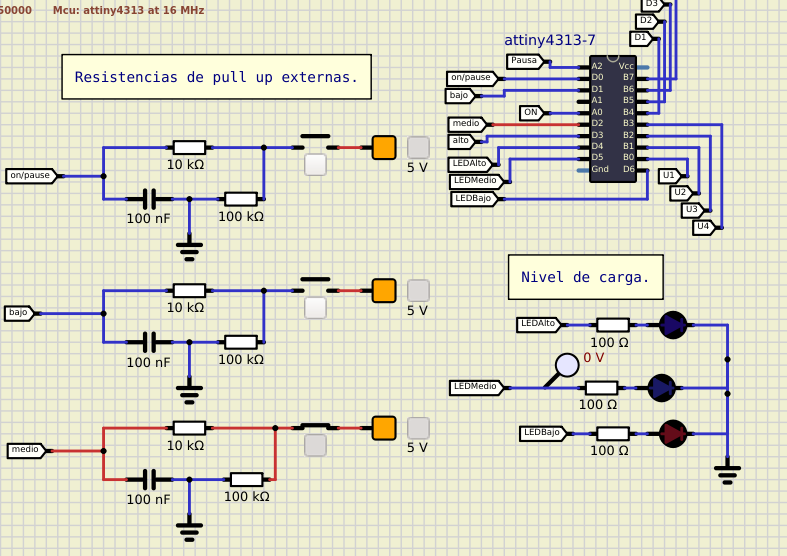
\includegraphics[width=.7\linewidth]{Imagenes/6.png}
     \caption{Carga media}\label{F12}
   \end{minipage}\hfill
   \begin{minipage}{0.48\textwidth}
     \centering
     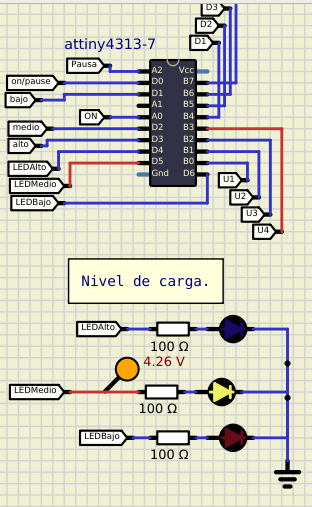
\includegraphics[width=.7\linewidth]{Imagenes/7.png}
     \caption{Indicador de carga media }\label{F13}
   \end{minipage}
\end{figure}
Primero se presiona el botón, donde es claro notar el flujo de corriente esperado que por medio de una interrupción le llegará al LED de carga media, y de manera inmediata es posible ver que el LED se enciende tal como se esperaba. Además, note que le está llegando una alimentación de \SI{5}{\volt}, lo que es una tensión eléctrica adecuada para que este componente no se dañe. Esta prueba se realizó con todos los demás LEDs.\par
Ahora, la segunda etapa consistió en mostrar en los displays de segmentos de la figura \ref{fig10} con los tiempos totales de cada carga que se le vaya asignar a la lavadora. Esto consiste en programar una cuenta regresiva haciendo uso de los pines B, los cuales están configurados como salida y así mostrar el respectivo número definido previamente en el código. Entonces, al presionar cualquiera de los 3 botones los display mostrarán el total del tiempo para cada carga tal como se muestra a continuación:
\begin{figure}[H]
        \centering
        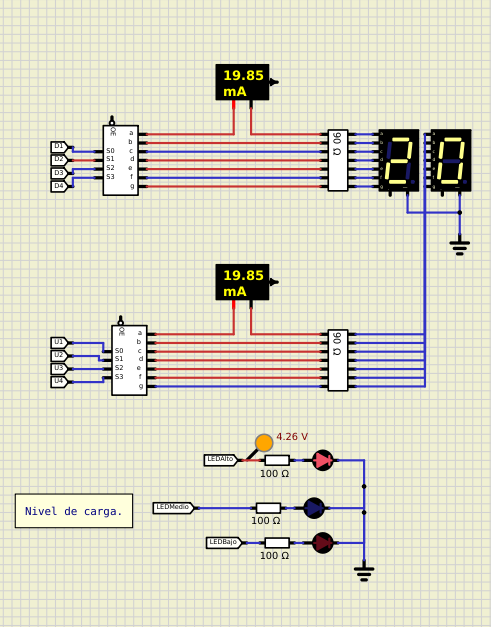
\includegraphics[width=.7\linewidth]{Imagenes/8.png}
        \caption{Encendido de un LED con cuenta regresiva.}
        \label{fig14}
    \end{figure}
Lo primero a resaltar es que la corriente eléctrica que le está llegando a los displays es la adecuada, ya que no supera los \SI{0.02}{\A}, así como al LED. Además, note que a los displays hay conectada una resistencia de \SI{90}{\ohm} para brindar protección a cada LED, esto justifica el hecho de no ver un parpadeo en cada segmento. Luego, el uso de las interrupciones para este caso (y los demás) presentan el resultado esperado a la hora de presionar el botón con carga alta.\par
Ahora, la siguiente prueba que se realizó fue la sincronización de los tiempos con los LEDs correspondientes para las 4 etapas de la lavadora. Esto por medio de una máquina de estados para realizar cada transición tal como se muestra en la figura \ref{fig15}.
\begin{figure}[H]
        \centering
        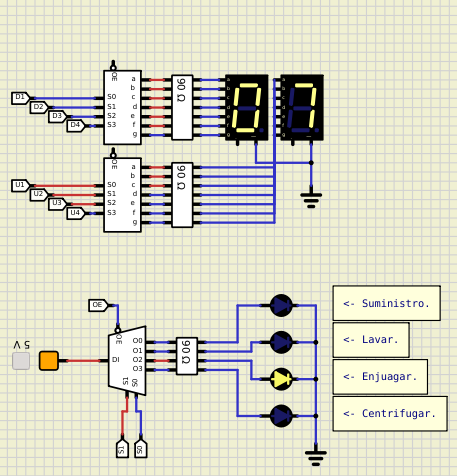
\includegraphics[width=.7\linewidth]{Imagenes/9.png}
        \caption{Transición de estados de la lavadora.}
        \label{fig15}
    \end{figure}
Hecho lo anterior, es posible ya mostrar el diseño completo del circuito que simula el comportamiento de una lavadora.
\begin{figure}[H]
        \centering
        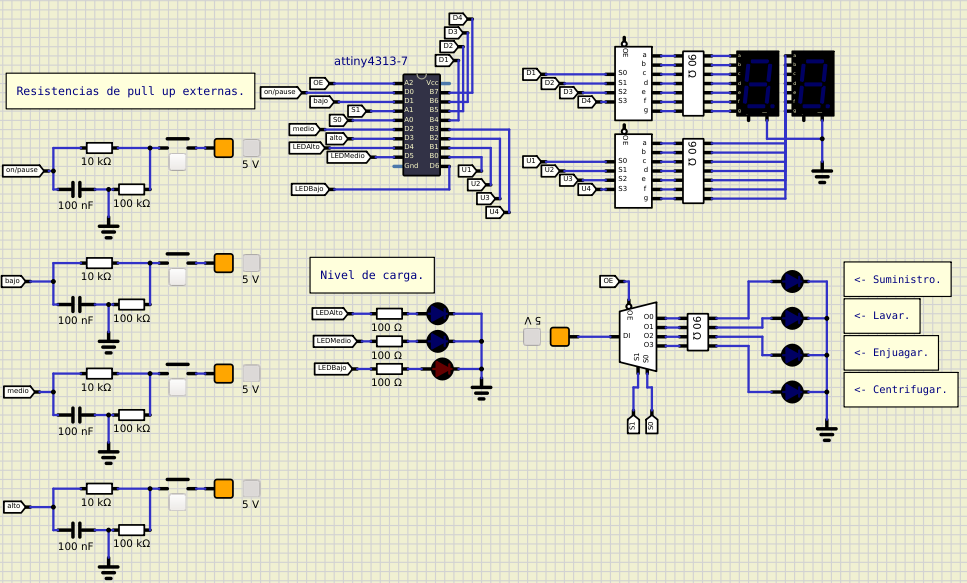
\includegraphics[width=.7\linewidth]{Imagenes/10.png}
        \caption{Diseño del circuito completo.}
        \label{fig16}
    \end{figure}
La programación de las funciones que hicieron este comportamiento posible se explicarán en la sección de resultados por medio de diagramas e imágenes. Por razones de tiempo, la última etapa del botón de pausa no se realizó, porque ya no hay más pines disponibles y se tendría que colocar un demultiplexor en alguna parte del circuito para lograr esto, eso implicaría muchos cambios en el código ya realizado.

\newpage


\section{Desarrollo/Análisis}
En esta sección, se hablará sobre las conexiones realizadas en el mcu y los diagramas de las principales funciones que componen el circuito de la lavadora.\par
Lo más sencillo fue declarar todos los pines B como salidas, porque es donde van conectados los Bcds en cascada con resistencias y los displays. Para declarar esos pines como salidas basta con escribir \texttt{DDRB = 0xff}. Ahora, con respecto a los botones, son partes del circuito que se encargarán de causar las interrupciones para hacer funcionar el circuito, en cuanto a la carga baja, media y alta, se conectaron a los pines D1, D2 y D3 respectivamente. A cada una de ellas fue necesario habilitar su comando de interrupción adecuado. Revisando la hoja del fabricante, para la carga baja, se debe habilitar el \texttt{PCMSK2} con el macro \texttt{PCINT12} y el \texttt{GIMSK} con el macro \texttt{PCIE2} para surtir efecto en este pin. En la carga media y alta, por medio de \texttt{GIMSK} se debe habilitar la interrupción con la macro \texttt{INTO} y \texttt{INT1}, esto hace que los botones trabajen apropiadamente. Ahora, en cuanto al \texttt{ISR} para cada uno de estos pines corresponden a las macros \texttt{PCINT2\_vect}, \texttt{INT0\_vect} y \texttt{INT1\_vect}. Dentro de estas interrupciones, hay una variable con el nombre: \texttt{tiempo\_inicio} que se iguala al tiempo total para cada carga, donde previamente se realizó un \texttt{\#define} con dichas magnitudes, además, se hace un llamado a la función \texttt{led\_carga} que se representa por el siguiente diagrama:
\begin{figure}[H]
    \centering
    



\tikzset{every picture/.style={line width=0.75pt}} %set default line width to 0.75pt        

\begin{tikzpicture}[x=0.75pt,y=0.75pt,yscale=-1,xscale=1]
%uncomment if require: \path (0,606); %set diagram left start at 0, and has height of 606

%Flowchart: Connector [id:dp021633046726569516] 
\draw   (290,58) .. controls (290,43.64) and (301.64,32) .. (316,32) .. controls (330.36,32) and (342,43.64) .. (342,58) .. controls (342,72.36) and (330.36,84) .. (316,84) .. controls (301.64,84) and (290,72.36) .. (290,58) -- cycle ;
%Flowchart: Decision [id:dp3699261934488949] 
\draw   (316,103) -- (375.25,150.5) -- (316,198) -- (256.75,150.5) -- cycle ;
%Straight Lines [id:da9331918609664245] 
\draw    (316,84) -- (316,100) ;
\draw [shift={(316,103)}, rotate = 270] [fill={rgb, 255:red, 0; green, 0; blue, 0 }  ][line width=0.08]  [draw opacity=0] (8.93,-4.29) -- (0,0) -- (8.93,4.29) -- cycle    ;
%Shape: Right Angle [id:dp2526929905854485] 
\draw   (375.25,150.5) -- (441,150.5) -- (441,176) ;
%Straight Lines [id:da07125413731798624] 
\draw    (441,176) -- (441,199) ;
\draw [shift={(441,202)}, rotate = 270] [fill={rgb, 255:red, 0; green, 0; blue, 0 }  ][line width=0.08]  [draw opacity=0] (8.93,-4.29) -- (0,0) -- (8.93,4.29) -- cycle    ;
%Flowchart: Process [id:dp7214387169012859] 
\draw   (391,200) -- (490,200) -- (490,245) -- (391,245) -- cycle ;
%Straight Lines [id:da2715179028720167] 
\draw    (316,198) -- (316,221) ;
\draw [shift={(316,224)}, rotate = 270] [fill={rgb, 255:red, 0; green, 0; blue, 0 }  ][line width=0.08]  [draw opacity=0] (8.93,-4.29) -- (0,0) -- (8.93,4.29) -- cycle    ;
%Flowchart: Process [id:dp9789563686318568] 
\draw   (366,440) -- (464,440) -- (464,491) -- (366,491) -- cycle ;
%Flowchart: Decision [id:dp1028100469525679] 
\draw   (316,224) -- (375.25,271.5) -- (316,319) -- (256.75,271.5) -- cycle ;
%Shape: Right Angle [id:dp7584861080562588] 
\draw   (256.75,271.5) -- (214,271.5) -- (214,294) ;
%Straight Lines [id:da2270209718957621] 
\draw    (415,413) -- (415,436) ;
\draw [shift={(415,439)}, rotate = 270] [fill={rgb, 255:red, 0; green, 0; blue, 0 }  ][line width=0.08]  [draw opacity=0] (8.93,-4.29) -- (0,0) -- (8.93,4.29) -- cycle    ;
%Straight Lines [id:da8351372179661163] 
\draw    (214,294) -- (214,317) ;
\draw [shift={(214,320)}, rotate = 270] [fill={rgb, 255:red, 0; green, 0; blue, 0 }  ][line width=0.08]  [draw opacity=0] (8.93,-4.29) -- (0,0) -- (8.93,4.29) -- cycle    ;
%Flowchart: Process [id:dp3175001957530377] 
\draw   (165,320) -- (265,320) -- (265,369) -- (165,369) -- cycle ;
%Straight Lines [id:da6198639865714966] 
\draw    (316,319) -- (316,342) ;
\draw [shift={(316,345)}, rotate = 270] [fill={rgb, 255:red, 0; green, 0; blue, 0 }  ][line width=0.08]  [draw opacity=0] (8.93,-4.29) -- (0,0) -- (8.93,4.29) -- cycle    ;
%Flowchart: Decision [id:dp2817555903877169] 
\draw   (316,345) -- (375.25,392.5) -- (316,440) -- (256.75,392.5) -- cycle ;
%Shape: Right Angle [id:dp6691165773669392] 
\draw   (375.25,392.5) -- (415,392.5) -- (415,413) ;
%Straight Lines [id:da7899754118364894] 
\draw    (316,440) -- (316.91,470) ;
\draw [shift={(317,473)}, rotate = 268.26] [fill={rgb, 255:red, 0; green, 0; blue, 0 }  ][line width=0.08]  [draw opacity=0] (8.93,-4.29) -- (0,0) -- (8.93,4.29) -- cycle    ;
%Flowchart: Connector [id:dp5690598454040376] 
\draw   (290,497) .. controls (290,482.64) and (301.64,471) .. (316,471) .. controls (330.36,471) and (342,482.64) .. (342,497) .. controls (342,511.36) and (330.36,523) .. (316,523) .. controls (301.64,523) and (290,511.36) .. (290,497) -- cycle ;

% Text Node
\draw (298,49) node [anchor=north west][inner sep=0.75pt]   [align=left] {Inicio};
% Text Node
\draw (273,141) node [anchor=north west][inner sep=0.75pt]   [align=left] {tiempo==alta};
% Text Node
\draw (263,261) node [anchor=north west][inner sep=0.75pt]   [align=left] {tiempo==media};
% Text Node
\draw (393,204) node [anchor=north west][inner sep=0.75pt]   [align=left] {LED PD4 ON\\estados()};
% Text Node
\draw (369,446) node [anchor=north west][inner sep=0.75pt]   [align=left] {LED PD6 ON\\estados()};
% Text Node
\draw (167,327) node [anchor=north west][inner sep=0.75pt]   [align=left] {LED PD5 ON\\estados()};
% Text Node
\draw (424,127) node [anchor=north west][inner sep=0.75pt]   [align=left] {Si};
% Text Node
\draw (286,208) node [anchor=north west][inner sep=0.75pt]   [align=left] {No};
% Text Node
\draw (291,321) node [anchor=north west][inner sep=0.75pt]   [align=left] {No};
% Text Node
\draw (274,382) node [anchor=north west][inner sep=0.75pt]   [align=left] {tiempo==alta};
% Text Node
\draw (399,372) node [anchor=north west][inner sep=0.75pt]   [align=left] {Si};
% Text Node
\draw (208,253) node [anchor=north west][inner sep=0.75pt]   [align=left] {Si};
% Text Node
\draw (308,488) node [anchor=north west][inner sep=0.75pt]   [align=left] {fin};


\end{tikzpicture}


\caption{Diagrama de flujo función led\_carga.}
\label{sch2}
\end{figure}
El diagrama anterior permite encender los LEDs con respecto al tiempo ya asignado en el enunciado del laboratorio, note que dentro de esta función hay un llamado a otra función: \texttt{estados}, esta es la máquina de estados para realizar la transición del encendido de los LEDs dependiendo si está en suministro, lavar, enjuague o centrifugar. El siguiente diagrama de flujo resume el comportamiento de esta función.
\begin{figure}[H]
    \centering


\tikzset{every picture/.style={line width=0.75pt}} %set default line width to 0.75pt        

\begin{tikzpicture}[x=0.75pt,y=0.75pt,yscale=-1,xscale=1]
%uncomment if require: \path (0,736); %set diagram left start at 0, and has height of 736

%Flowchart: Connector [id:dp12439739573210629] 
\draw   (355,32) .. controls (355,17.64) and (366.64,6) .. (381,6) .. controls (395.36,6) and (407,17.64) .. (407,32) .. controls (407,46.36) and (395.36,58) .. (381,58) .. controls (366.64,58) and (355,46.36) .. (355,32) -- cycle ;
%Straight Lines [id:da0911199105915208] 
\draw    (381,58) -- (381,74) ;
\draw [shift={(381,77)}, rotate = 270] [fill={rgb, 255:red, 0; green, 0; blue, 0 }  ][line width=0.08]  [draw opacity=0] (8.93,-4.29) -- (0,0) -- (8.93,4.29) -- cycle    ;
%Flowchart: Process [id:dp6149465951989119] 
\draw   (47,123) -- (100,123) -- (100,154.33) -- (47,154.33) -- cycle ;
%Straight Lines [id:da8868380418121589] 
\draw    (74,110) -- (74,120) ;
\draw [shift={(74,123)}, rotate = 270] [fill={rgb, 255:red, 0; green, 0; blue, 0 }  ][line width=0.08]  [draw opacity=0] (8.93,-4.29) -- (0,0) -- (8.93,4.29) -- cycle    ;
%Shape: Right Angle [id:dp6906836722085405] 
\draw   (475.75,141.5) -- (463,141.5) -- (463,168) ;
%Straight Lines [id:da12005298293316646] 
\draw    (463,168) -- (463,191) ;
\draw [shift={(463,194)}, rotate = 270] [fill={rgb, 255:red, 0; green, 0; blue, 0 }  ][line width=0.08]  [draw opacity=0] (8.93,-4.29) -- (0,0) -- (8.93,4.29) -- cycle    ;
%Flowchart: Process [id:dp4261666254360057] 
\draw   (432,193) -- (498,193) -- (498,221) -- (432,221) -- cycle ;
%Straight Lines [id:da019990857102445414] 
\draw    (579,164) -- (579,187) ;
\draw [shift={(579,190)}, rotate = 270] [fill={rgb, 255:red, 0; green, 0; blue, 0 }  ][line width=0.08]  [draw opacity=0] (8.93,-4.29) -- (0,0) -- (8.93,4.29) -- cycle    ;
%Shape: Right Angle [id:dp6724134432403848] 
\draw   (408,93) -- (484,93) -- (484,111) ;
%Straight Lines [id:da7874407775672443] 
\draw    (484,111) -- (511,110.1) ;
\draw [shift={(514,110)}, rotate = 178.09] [fill={rgb, 255:red, 0; green, 0; blue, 0 }  ][line width=0.08]  [draw opacity=0] (8.93,-4.29) -- (0,0) -- (8.93,4.29) -- cycle    ;
%Shape: Right Angle [id:dp1803471909800265] 
\draw   (553.25,142.5) -- (579,142.5) -- (579,164) ;
%Flowchart: Decision [id:dp8940401462112177] 
\draw   (580,189) -- (639.25,236.5) -- (580,284) -- (520.75,236.5) -- cycle ;
%Shape: Right Angle [id:dp9888575078003836] 
\draw   (520.75,236.5) -- (508,236.5) -- (508,263) ;
%Straight Lines [id:da9039594504404762] 
\draw    (508,263) -- (492,262.16) ;
\draw [shift={(489,262)}, rotate = 3.01] [fill={rgb, 255:red, 0; green, 0; blue, 0 }  ][line width=0.08]  [draw opacity=0] (8.93,-4.29) -- (0,0) -- (8.93,4.29) -- cycle    ;
%Flowchart: Process [id:dp1878281348761568] 
\draw   (423,248) -- (491,248) -- (491,275) -- (423,275) -- cycle ;
%Straight Lines [id:da7045473332712788] 
\draw    (580,284) -- (580,307) ;
\draw [shift={(580,310)}, rotate = 270] [fill={rgb, 255:red, 0; green, 0; blue, 0 }  ][line width=0.08]  [draw opacity=0] (8.93,-4.29) -- (0,0) -- (8.93,4.29) -- cycle    ;
%Flowchart: Decision [id:dp7590302190788398] 
\draw   (580,308) -- (639.25,355.5) -- (580,403) -- (520.75,355.5) -- cycle ;
%Shape: Right Angle [id:dp21013725002314598] 
\draw   (520.75,355.5) -- (508,355.5) -- (508,382) ;
%Straight Lines [id:da9648131280624423] 
\draw    (508,382) -- (492,381.16) ;
\draw [shift={(489,381)}, rotate = 3.01] [fill={rgb, 255:red, 0; green, 0; blue, 0 }  ][line width=0.08]  [draw opacity=0] (8.93,-4.29) -- (0,0) -- (8.93,4.29) -- cycle    ;
%Flowchart: Process [id:dp9160651251463305] 
\draw   (389,367) -- (489,367) -- (489,397) -- (389,397) -- cycle ;
%Straight Lines [id:da8522104020423502] 
\draw    (580,403) -- (580,426) ;
\draw [shift={(580,429)}, rotate = 270] [fill={rgb, 255:red, 0; green, 0; blue, 0 }  ][line width=0.08]  [draw opacity=0] (8.93,-4.29) -- (0,0) -- (8.93,4.29) -- cycle    ;
%Flowchart: Decision [id:dp12658023343568292] 
\draw   (580,429) -- (639.25,476.5) -- (580,524) -- (520.75,476.5) -- cycle ;
%Shape: Right Angle [id:dp134629382260554] 
\draw   (520.75,476.5) -- (508,476.5) -- (508,503) ;
%Straight Lines [id:da02925904812151492] 
\draw    (508,503) -- (492,502.16) ;
\draw [shift={(489,502)}, rotate = 3.01] [fill={rgb, 255:red, 0; green, 0; blue, 0 }  ][line width=0.08]  [draw opacity=0] (8.93,-4.29) -- (0,0) -- (8.93,4.29) -- cycle    ;
%Flowchart: Process [id:dp9433679378308446] 
\draw   (417,490) -- (488,490) -- (488,517) -- (417,517) -- cycle ;
%Straight Lines [id:da26870518401603505] 
\draw    (580,524) -- (580,547) ;
\draw [shift={(580,550)}, rotate = 270] [fill={rgb, 255:red, 0; green, 0; blue, 0 }  ][line width=0.08]  [draw opacity=0] (8.93,-4.29) -- (0,0) -- (8.93,4.29) -- cycle    ;
%Flowchart: Process [id:dp9811382267708229] 
\draw   (550,550) -- (607,550) -- (607,580) -- (550,580) -- cycle ;
%Shape: Right Angle [id:dp8598411976781433] 
\draw   (354,92) -- (74,92) -- (74,110) ;
%Flowchart: Decision [id:dp21488379209338482] 
\draw   (75.42,173.67) -- (114,204.83) -- (75.42,236) -- (36.83,204.83) -- cycle ;
%Shape: Right Angle [id:dp26291738895516636] 
\draw   (36.83,204.83) -- (24,204.83) -- (24,216) ;
%Straight Lines [id:da6659896216340511] 
\draw    (24,216) -- (24,239) ;
\draw [shift={(24,242)}, rotate = 270] [fill={rgb, 255:red, 0; green, 0; blue, 0 }  ][line width=0.08]  [draw opacity=0] (8.93,-4.29) -- (0,0) -- (8.93,4.29) -- cycle    ;
%Flowchart: Process [id:dp23715148378192508] 
\draw   (6,242) -- (72,242) -- (72,259.81) -- (6,259.81) -- cycle ;
%Straight Lines [id:da7175092852653877] 
\draw    (139,217) -- (139,240) ;
\draw [shift={(139,243)}, rotate = 270] [fill={rgb, 255:red, 0; green, 0; blue, 0 }  ][line width=0.08]  [draw opacity=0] (8.93,-4.29) -- (0,0) -- (8.93,4.29) -- cycle    ;
%Shape: Right Angle [id:dp7282756797126677] 
\draw   (114,204.83) -- (139,204.83) -- (139,217) ;
%Flowchart: Decision [id:dp679752545363411] 
\draw   (139,243) -- (198.25,270.5) -- (139,298) -- (79.75,270.5) -- cycle ;
%Shape: Right Angle [id:dp8761291449153592] 
\draw   (79.75,270.5) -- (67,270.5) -- (67,297) ;
%Straight Lines [id:da9650771288485256] 
\draw    (67,297) -- (67,305) ;
\draw [shift={(67,308)}, rotate = 270] [fill={rgb, 255:red, 0; green, 0; blue, 0 }  ][line width=0.08]  [draw opacity=0] (8.93,-4.29) -- (0,0) -- (8.93,4.29) -- cycle    ;
%Flowchart: Process [id:dp6312403338347992] 
\draw   (34,306.67) -- (104,306.67) -- (104,335) -- (34,335) -- cycle ;
%Straight Lines [id:da35042274703091447] 
\draw    (139,298) -- (138.07,339) ;
\draw [shift={(138,342)}, rotate = 271.3] [fill={rgb, 255:red, 0; green, 0; blue, 0 }  ][line width=0.08]  [draw opacity=0] (8.93,-4.29) -- (0,0) -- (8.93,4.29) -- cycle    ;
%Flowchart: Decision [id:dp2936421274241927] 
\draw   (138.08,342) -- (197.33,370.5) -- (138.08,399) -- (78.83,370.5) -- cycle ;
%Shape: Right Angle [id:dp42175811220875525] 
\draw   (80.83,370.17) -- (69,370.17) -- (69,384) ;
%Straight Lines [id:da36210638117227556] 
\draw    (69,384) -- (68.93,400.33) ;
\draw [shift={(68.92,403.33)}, rotate = 270.25] [fill={rgb, 255:red, 0; green, 0; blue, 0 }  ][line width=0.08]  [draw opacity=0] (8.93,-4.29) -- (0,0) -- (8.93,4.29) -- cycle    ;
%Flowchart: Process [id:dp06368758111530282] 
\draw   (22.08,402.67) -- (122.08,402.67) -- (122.08,432.67) -- (22.08,432.67) -- cycle ;
%Straight Lines [id:da6829150776274491] 
\draw    (138.08,399) -- (138.01,440) ;
\draw [shift={(138,443)}, rotate = 270.11] [fill={rgb, 255:red, 0; green, 0; blue, 0 }  ][line width=0.08]  [draw opacity=0] (8.93,-4.29) -- (0,0) -- (8.93,4.29) -- cycle    ;
%Flowchart: Decision [id:dp21332806721811415] 
\draw   (138,443) -- (197.25,467.83) -- (138,492.67) -- (78.75,467.83) -- cycle ;
%Shape: Right Angle [id:dp8939949854170095] 
\draw   (78.75,467.83) -- (73,467.83) -- (73,496) ;
%Straight Lines [id:da9774114081951284] 
\draw    (73,496) -- (73,508) ;
\draw [shift={(73,511)}, rotate = 270] [fill={rgb, 255:red, 0; green, 0; blue, 0 }  ][line width=0.08]  [draw opacity=0] (8.93,-4.29) -- (0,0) -- (8.93,4.29) -- cycle    ;
%Flowchart: Process [id:dp775718312939818] 
\draw   (35.08,509.67) -- (108,509.67) -- (108,536) -- (35.08,536) -- cycle ;
%Straight Lines [id:da016170408812257175] 
\draw    (138,492.67) -- (138.94,540) ;
\draw [shift={(139,543)}, rotate = 268.86] [fill={rgb, 255:red, 0; green, 0; blue, 0 }  ][line width=0.08]  [draw opacity=0] (8.93,-4.29) -- (0,0) -- (8.93,4.29) -- cycle    ;
%Flowchart: Decision [id:dp3953876048094218] 
\draw   (514.42,110.67) -- (553,141.83) -- (514.42,173) -- (475.83,141.83) -- cycle ;
%Straight Lines [id:da4743960354930279] 
\draw    (75,155) -- (75,171) ;
\draw [shift={(75,174)}, rotate = 270] [fill={rgb, 255:red, 0; green, 0; blue, 0 }  ][line width=0.08]  [draw opacity=0] (8.93,-4.29) -- (0,0) -- (8.93,4.29) -- cycle    ;
%Shape: Right Angle [id:dp8466659682561892] 
\draw   (100,139.67) -- (315,139.67) -- (315,194) ;
%Straight Lines [id:da4649712336561458] 
\draw    (315,194) -- (315,212) ;
\draw [shift={(315,215)}, rotate = 270] [fill={rgb, 255:red, 0; green, 0; blue, 0 }  ][line width=0.08]  [draw opacity=0] (8.93,-4.29) -- (0,0) -- (8.93,4.29) -- cycle    ;
%Flowchart: Process [id:dp8283630291095716] 
\draw   (288,215.33) -- (341,215.33) -- (341,246.67) -- (288,246.67) -- cycle ;
%Flowchart: Process [id:dp4922525180421693] 
\draw   (355,76) -- (408,76) -- (408,107.33) -- (355,107.33) -- cycle ;
%Straight Lines [id:da28645691514326366] 
\draw    (316,246) -- (316.89,271) ;
\draw [shift={(317,274)}, rotate = 267.95] [fill={rgb, 255:red, 0; green, 0; blue, 0 }  ][line width=0.08]  [draw opacity=0] (8.93,-4.29) -- (0,0) -- (8.93,4.29) -- cycle    ;
%Flowchart: Connector [id:dp6291119086530925] 
\draw   (291,300) .. controls (291,285.64) and (302.64,274) .. (317,274) .. controls (331.36,274) and (343,285.64) .. (343,300) .. controls (343,314.36) and (331.36,326) .. (317,326) .. controls (302.64,326) and (291,314.36) .. (291,300) -- cycle ;
%Flowchart: Process [id:dp4549925468032834] 
\draw   (110,543) -- (167,543) -- (167,573) -- (110,573) -- cycle ;

% Text Node
\draw (363,23) node [anchor=north west][inner sep=0.75pt]   [align=left] {Inicio};
% Text Node
\draw (362,84) node [anchor=north west][inner sep=0.75pt]   [align=left] {baja};
% Text Node
\draw (302.33,220.67) node [anchor=north west][inner sep=0.75pt]   [align=left] {alta};
% Text Node
\draw (52.14,130.97) node [anchor=north west][inner sep=0.75pt]   [align=left] {media};
% Text Node
\draw (433,198) node [anchor=north west][inner sep=0.75pt]   [align=left] {Sumi ON};
% Text Node
\draw (72,72) node [anchor=north west][inner sep=0.75pt]   [align=left] {No};
% Text Node
\draw (564,124) node [anchor=north west][inner sep=0.75pt]   [align=left] {No};
% Text Node
\draw (505,218) node [anchor=north west][inner sep=0.75pt]   [align=left] {Si};
% Text Node
\draw (358,57) node [anchor=north west][inner sep=0.75pt]   [align=left] {Si};
% Text Node
\draw (454,122) node [anchor=north west][inner sep=0.75pt]   [align=left] {Si};
% Text Node
\draw (535,227) node [anchor=north west][inner sep=0.75pt]   [align=left] {$\displaystyle 1\leqslant $seg$\displaystyle < 7$};
% Text Node
\draw (412,252) node [anchor=north west][inner sep=0.75pt]   [align=left] { \ \ Lavar ON};
% Text Node
\draw (585,279) node [anchor=north west][inner sep=0.75pt]   [align=left] {No};
% Text Node
\draw (536,346) node [anchor=north west][inner sep=0.75pt]   [align=left] {$\displaystyle 4< $seg$\displaystyle < 7$};
% Text Node
\draw (391,373) node [anchor=north west][inner sep=0.75pt]   [align=left] {Enjuague ON};
% Text Node
\draw (514,331) node [anchor=north west][inner sep=0.75pt]   [align=left] {Si};
% Text Node
\draw (585,399) node [anchor=north west][inner sep=0.75pt]   [align=left] {No};
% Text Node
\draw (533,466) node [anchor=north west][inner sep=0.75pt]   [align=left] {$\displaystyle 7\leqslant $seg$\displaystyle < ...$};
% Text Node
\draw (419,496) node [anchor=north west][inner sep=0.75pt]   [align=left] {Centri ON};
% Text Node
\draw (511,453) node [anchor=north west][inner sep=0.75pt]   [align=left] {Si};
% Text Node
\draw (584,521) node [anchor=north west][inner sep=0.75pt]   [align=left] {No};
% Text Node
\draw (551,554) node [anchor=north west][inner sep=0.75pt]   [align=left] {Led\_off};
% Text Node
\draw (50.08,194.67) node [anchor=north west][inner sep=0.75pt]   [align=left] {seg==0};
% Text Node
\draw (7.08,240.5) node [anchor=north west][inner sep=0.75pt]   [align=left] {Sumi ON};
% Text Node
\draw (120.08,184.67) node [anchor=north west][inner sep=0.75pt]   [align=left] {No};
% Text Node
\draw (73.08,273.67) node [anchor=north west][inner sep=0.75pt]   [align=left] {Si};
% Text Node
\draw (29.08,182.67) node [anchor=north west][inner sep=0.75pt]   [align=left] {Si};
% Text Node
\draw (96.08,259.67) node [anchor=north west][inner sep=0.75pt]   [align=left] {$\displaystyle 2\leqslant $seg$\displaystyle < 8$};
% Text Node
\draw (24.08,310.67) node [anchor=north west][inner sep=0.75pt]   [align=left] { \ \ Lavar ON};
% Text Node
\draw (143.08,295.67) node [anchor=north west][inner sep=0.75pt]   [align=left] {No};
% Text Node
\draw (91.08,360.67) node [anchor=north west][inner sep=0.75pt]   [align=left] {$\displaystyle 8\leqslant $seg$\displaystyle < 13$};
% Text Node
\draw (24.08,408.67) node [anchor=north west][inner sep=0.75pt]   [align=left] {Enjuague ON};
% Text Node
\draw (60.08,352.67) node [anchor=north west][inner sep=0.75pt]   [align=left] {Si};
% Text Node
\draw (143.08,395.67) node [anchor=north west][inner sep=0.75pt]   [align=left] {No};
% Text Node
\draw (94.08,458.67) node [anchor=north west][inner sep=0.75pt]   [align=left] {$\displaystyle 13\leqslant $seg$\displaystyle < ...$};
% Text Node
\draw (33.08,515.67) node [anchor=north west][inner sep=0.75pt]   [align=left] {Centri ON};
% Text Node
\draw (65.08,447.67) node [anchor=north west][inner sep=0.75pt]   [align=left] {Si};
% Text Node
\draw (147.08,492.67) node [anchor=north west][inner sep=0.75pt]   [align=left] {No};
% Text Node
\draw (486.08,130.67) node [anchor=north west][inner sep=0.75pt]   [align=left] {seg==0};
% Text Node
\draw (297,290) node [anchor=north west][inner sep=0.75pt]   [align=left] {Label};
% Text Node
\draw (111,547) node [anchor=north west][inner sep=0.75pt]   [align=left] {Led\_off};
% Text Node
\draw (470,74) node [anchor=north west][inner sep=0.75pt]   [align=left] {Si};
% Text Node
\draw (84,152) node [anchor=north west][inner sep=0.75pt]   [align=left] {Si};
% Text Node
\draw (295,120) node [anchor=north west][inner sep=0.75pt]   [align=left] {No};
% Text Node
\draw (296,249) node [anchor=north west][inner sep=0.75pt]   [align=left] {Si};


\end{tikzpicture}

\caption{Máquina de estados transición de LEDs.}
\label{sch3}
\end{figure}
\begin{figure}[H]
    \centering



\tikzset{every picture/.style={line width=0.75pt}} %set default line width to 0.75pt        

\begin{tikzpicture}[x=0.75pt,y=0.75pt,yscale=-1,xscale=1]
%uncomment if require: \path (0,501); %set diagram left start at 0, and has height of 501

%Flowchart: Connector [id:dp86445783611407] 
\draw   (280,41) .. controls (280,26.64) and (291.64,15) .. (306,15) .. controls (320.36,15) and (332,26.64) .. (332,41) .. controls (332,55.36) and (320.36,67) .. (306,67) .. controls (291.64,67) and (280,55.36) .. (280,41) -- cycle ;
%Flowchart: Decision [id:dp935312970889731] 
\draw   (306.33,85.67) -- (344.92,116.83) -- (306.33,148) -- (267.75,116.83) -- cycle ;
%Shape: Right Angle [id:dp07822486648512661] 
\draw   (267.75,116.83) -- (254.92,116.83) -- (254.92,128) ;
%Straight Lines [id:da37127883940863304] 
\draw    (254.92,128) -- (254.92,151) ;
\draw [shift={(254.92,154)}, rotate = 270] [fill={rgb, 255:red, 0; green, 0; blue, 0 }  ][line width=0.08]  [draw opacity=0] (8.93,-4.29) -- (0,0) -- (8.93,4.29) -- cycle    ;
%Flowchart: Process [id:dp4908952967414264] 
\draw   (236.92,154) -- (302.92,154) -- (302.92,171.81) -- (236.92,171.81) -- cycle ;
%Straight Lines [id:da7626068450578292] 
\draw    (369.92,129) -- (369.92,152) ;
\draw [shift={(369.92,155)}, rotate = 270] [fill={rgb, 255:red, 0; green, 0; blue, 0 }  ][line width=0.08]  [draw opacity=0] (8.93,-4.29) -- (0,0) -- (8.93,4.29) -- cycle    ;
%Shape: Right Angle [id:dp1235200916676118] 
\draw   (344.92,116.83) -- (369.92,116.83) -- (369.92,129) ;
%Flowchart: Decision [id:dp0636696577602811] 
\draw   (369.92,155) -- (429.17,182.5) -- (369.92,210) -- (310.67,182.5) -- cycle ;
%Shape: Right Angle [id:dp25067118553920165] 
\draw   (310.67,182.5) -- (297.92,182.5) -- (297.92,209) ;
%Straight Lines [id:da7947446829986125] 
\draw    (297.92,209) -- (297.92,217) ;
\draw [shift={(297.92,220)}, rotate = 270] [fill={rgb, 255:red, 0; green, 0; blue, 0 }  ][line width=0.08]  [draw opacity=0] (8.93,-4.29) -- (0,0) -- (8.93,4.29) -- cycle    ;
%Flowchart: Process [id:dp8895352375244476] 
\draw   (264.92,218.67) -- (334.92,218.67) -- (334.92,247) -- (264.92,247) -- cycle ;
%Straight Lines [id:da9249878842399695] 
\draw    (369.92,210) -- (368.98,251) ;
\draw [shift={(368.92,254)}, rotate = 271.3] [fill={rgb, 255:red, 0; green, 0; blue, 0 }  ][line width=0.08]  [draw opacity=0] (8.93,-4.29) -- (0,0) -- (8.93,4.29) -- cycle    ;
%Flowchart: Decision [id:dp027950767579304037] 
\draw   (369,254) -- (428.25,282.5) -- (369,311) -- (309.75,282.5) -- cycle ;
%Shape: Right Angle [id:dp7113899430080068] 
\draw   (311.75,282.17) -- (299.92,282.17) -- (299.92,296) ;
%Straight Lines [id:da6331255525268646] 
\draw    (299.92,296) -- (299.85,312.33) ;
\draw [shift={(299.83,315.33)}, rotate = 270.25] [fill={rgb, 255:red, 0; green, 0; blue, 0 }  ][line width=0.08]  [draw opacity=0] (8.93,-4.29) -- (0,0) -- (8.93,4.29) -- cycle    ;
%Flowchart: Process [id:dp31180552945320983] 
\draw   (253,314.67) -- (353,314.67) -- (353,344.67) -- (253,344.67) -- cycle ;
%Straight Lines [id:da1282233954801908] 
\draw    (369,311) -- (368.92,352) ;
\draw [shift={(368.92,355)}, rotate = 270.11] [fill={rgb, 255:red, 0; green, 0; blue, 0 }  ][line width=0.08]  [draw opacity=0] (8.93,-4.29) -- (0,0) -- (8.93,4.29) -- cycle    ;
%Flowchart: Decision [id:dp5974483452503938] 
\draw   (368.92,355) -- (428.17,379.83) -- (368.92,404.67) -- (309.67,379.83) -- cycle ;
%Shape: Right Angle [id:dp3217161793632042] 
\draw   (309.67,379.83) -- (303.92,379.83) -- (303.92,408) ;
%Straight Lines [id:da6569908124389181] 
\draw    (303.92,408) -- (303.92,420) ;
\draw [shift={(303.92,423)}, rotate = 270] [fill={rgb, 255:red, 0; green, 0; blue, 0 }  ][line width=0.08]  [draw opacity=0] (8.93,-4.29) -- (0,0) -- (8.93,4.29) -- cycle    ;
%Flowchart: Process [id:dp9233334167885809] 
\draw   (266,421.67) -- (338.92,421.67) -- (338.92,448) -- (266,448) -- cycle ;
%Straight Lines [id:da0014516432713123084] 
\draw    (368.92,404.67) -- (369.86,452) ;
\draw [shift={(369.92,455)}, rotate = 268.86] [fill={rgb, 255:red, 0; green, 0; blue, 0 }  ][line width=0.08]  [draw opacity=0] (8.93,-4.29) -- (0,0) -- (8.93,4.29) -- cycle    ;
%Straight Lines [id:da24463353428391343] 
\draw    (305.92,67) -- (305.92,83) ;
\draw [shift={(305.92,86)}, rotate = 270] [fill={rgb, 255:red, 0; green, 0; blue, 0 }  ][line width=0.08]  [draw opacity=0] (8.93,-4.29) -- (0,0) -- (8.93,4.29) -- cycle    ;
%Flowchart: Process [id:dp8528821341043025] 
\draw   (340.92,455) -- (397.92,455) -- (397.92,485) -- (340.92,485) -- cycle ;

% Text Node
\draw (286,31) node [anchor=north west][inner sep=0.75pt]   [align=left] {Label};
% Text Node
\draw (281,106.67) node [anchor=north west][inner sep=0.75pt]   [align=left] {seg==0};
% Text Node
\draw (238,152.5) node [anchor=north west][inner sep=0.75pt]   [align=left] {Sumi ON};
% Text Node
\draw (351,96.67) node [anchor=north west][inner sep=0.75pt]   [align=left] {No};
% Text Node
\draw (304,185.67) node [anchor=north west][inner sep=0.75pt]   [align=left] {Si};
% Text Node
\draw (260,94.67) node [anchor=north west][inner sep=0.75pt]   [align=left] {Si};
% Text Node
\draw (324,172.67) node [anchor=north west][inner sep=0.75pt]   [align=left] {$\displaystyle 3\leqslant $seg$\displaystyle < 13$};
% Text Node
\draw (255,222.67) node [anchor=north west][inner sep=0.75pt]   [align=left] { \ \ Lavar ON};
% Text Node
\draw (374,207.67) node [anchor=north west][inner sep=0.75pt]   [align=left] {No};
% Text Node
\draw (319,272.67) node [anchor=north west][inner sep=0.75pt]   [align=left] {$\displaystyle 14< $seg$\displaystyle < 19$};
% Text Node
\draw (255,320.67) node [anchor=north west][inner sep=0.75pt]   [align=left] {Enjuague ON};
% Text Node
\draw (291,264.67) node [anchor=north west][inner sep=0.75pt]   [align=left] {Si};
% Text Node
\draw (374,307.67) node [anchor=north west][inner sep=0.75pt]   [align=left] {No};
% Text Node
\draw (325,366.67) node [anchor=north west][inner sep=0.75pt]   [align=left] {$\displaystyle 19\leqslant $seg$\displaystyle < ...$};
% Text Node
\draw (268,427.67) node [anchor=north west][inner sep=0.75pt]   [align=left] {Centri ON};
% Text Node
\draw (296,359.67) node [anchor=north west][inner sep=0.75pt]   [align=left] {Si};
% Text Node
\draw (378,404.67) node [anchor=north west][inner sep=0.75pt]   [align=left] {No};
% Text Node
\draw (341.92,459) node [anchor=north west][inner sep=0.75pt]   [align=left] {Led\_off};
% Text Node
\draw (314.92,64) node [anchor=north west][inner sep=0.75pt]   [align=left] {Si};


\end{tikzpicture}


\caption{Conituación máquina de estados transición de LEDs.}
\label{sch3.1}
\end{figure}
Esta máquina de estados se encarga de administrar los tiempos para cada carga, por lo que se define un intervalo de tiempo para cada etapa, esto con base al tiempo ya establecido. Entonces, una vez que se cumple cada desigualdad, se apaga el LED actual y se enciende el siguiente LED con el estado correspondiente. Esto para cada situación, dependiendo de la carga que se le asigne a la lavadora. Ahora, hay dos detalles en esta máquina de estados, lo primero es que para referescar los LEDs se hace uso de la interrupción \texttt{TIMER0\_COMPA\_vect} y esto con base al tiempo asignado, esto permite también llevar una cuenta de los segundos que pasan. Claramente hay que hacer las configuraciones para lograr esto, lo primero es con  \texttt{TCCR0A} y la macro \texttt{WGM12}, luego la variable \texttt{OCR1A} para obtener un 1 segundo, el prescaler de 256 y habilitar la interrupción. Esta interrupción se compone de una función: \texttt{display}, la cual es encargada de mostrar la cuenta regresiva de los números mostrados en los displays, el diagrama de flujo de esta función se muestra a continuación,

\begin{figure}[H]
    \centering



\tikzset{every picture/.style={line width=0.75pt}} %set default line width to 0.75pt        

\begin{tikzpicture}[x=0.75pt,y=0.75pt,yscale=-1,xscale=1]
%uncomment if require: \path (0,649); %set diagram left start at 0, and has height of 649

%Flowchart: Connector [id:dp42585090626324207] 
\draw   (300,61) .. controls (300,46.64) and (311.64,35) .. (326,35) .. controls (340.36,35) and (352,46.64) .. (352,61) .. controls (352,75.36) and (340.36,87) .. (326,87) .. controls (311.64,87) and (300,75.36) .. (300,61) -- cycle ;
%Straight Lines [id:da9927818650372262] 
\draw    (325.92,87) -- (325.92,103) ;
\draw [shift={(325.92,106)}, rotate = 270] [fill={rgb, 255:red, 0; green, 0; blue, 0 }  ][line width=0.08]  [draw opacity=0] (8.93,-4.29) -- (0,0) -- (8.93,4.29) -- cycle    ;
%Flowchart: Decision [id:dp8222109791046812] 
\draw   (325.92,106) -- (364.5,137.17) -- (325.92,168.33) -- (287.33,137.17) -- cycle ;
%Shape: Right Angle [id:dp5468713947182464] 
\draw   (287.33,137.17) -- (241,137.17) -- (241,158) ;
%Straight Lines [id:da34123972616362797] 
\draw    (241,158) -- (241.87,178) ;
\draw [shift={(242,181)}, rotate = 267.51] [fill={rgb, 255:red, 0; green, 0; blue, 0 }  ][line width=0.08]  [draw opacity=0] (8.93,-4.29) -- (0,0) -- (8.93,4.29) -- cycle    ;
%Flowchart: Process [id:dp6422094052668206] 
\draw   (199,181) -- (287,181) -- (287,239) -- (199,239) -- cycle ;
%Shape: Right Angle [id:dp9632380337734168] 
\draw   (364.5,137.17) -- (409,137.17) -- (409,159) ;
%Straight Lines [id:da9224648988654192] 
\draw    (409,159) -- (409.87,179) ;
\draw [shift={(410,182)}, rotate = 267.51] [fill={rgb, 255:red, 0; green, 0; blue, 0 }  ][line width=0.08]  [draw opacity=0] (8.93,-4.29) -- (0,0) -- (8.93,4.29) -- cycle    ;
%Flowchart: Process [id:dp38544924804806135] 
\draw   (368,182) -- (450,182) -- (450,213) -- (368,213) -- cycle ;
%Straight Lines [id:da9362534173457413] 
\draw    (407,214) -- (407.89,239) ;
\draw [shift={(408,242)}, rotate = 267.95] [fill={rgb, 255:red, 0; green, 0; blue, 0 }  ][line width=0.08]  [draw opacity=0] (8.93,-4.29) -- (0,0) -- (8.93,4.29) -- cycle    ;
%Flowchart: Process [id:dp015535025341874897] 
\draw   (380,243) -- (438,243) -- (438,275) -- (380,275) -- cycle ;
%Straight Lines [id:da14093121348085114] 
\draw    (408,276) -- (408.89,301) ;
\draw [shift={(409,304)}, rotate = 267.95] [fill={rgb, 255:red, 0; green, 0; blue, 0 }  ][line width=0.08]  [draw opacity=0] (8.93,-4.29) -- (0,0) -- (8.93,4.29) -- cycle    ;
%Flowchart: Connector [id:dp28231580529895073] 
\draw   (383,330) .. controls (383,315.64) and (394.64,304) .. (409,304) .. controls (423.36,304) and (435,315.64) .. (435,330) .. controls (435,344.36) and (423.36,356) .. (409,356) .. controls (394.64,356) and (383,344.36) .. (383,330) -- cycle ;

% Text Node
\draw (309,51) node [anchor=north west][inner sep=0.75pt]   [align=left] {Inicio};
% Text Node
\draw (229.92,116) node [anchor=north west][inner sep=0.75pt]   [align=left] {Si};
% Text Node
\draw (299.08,126.67) node [anchor=north west][inner sep=0.75pt]   [align=left] {temp!=0};
% Text Node
\draw (201,184) node [anchor=north west][inner sep=0.75pt]   [align=left] {u=temp\%10\\d =temp/10};
% Text Node
\draw (392.92,117) node [anchor=north west][inner sep=0.75pt]   [align=left] {No};
% Text Node
\draw (372.08,190.67) node [anchor=north west][inner sep=0.75pt]   [align=left] {Mostrar 0's};
% Text Node
\draw (386,251) node [anchor=north west][inner sep=0.75pt]   [align=left] {RESET};
% Text Node
\draw (401,320) node [anchor=north west][inner sep=0.75pt]   [align=left] {fin};


\end{tikzpicture}

    \caption{Función display}
    \label{FigWW}
\end{figure}

de donde primero se define la varible como la resta de esta misma variable con segundos, luego con ayuda de condicional se comprueba que el tiempo de carga no sea 0 para poder separar unidades y decenas del número, así, se toman los 4 bits LSB y se colocan en las unidades, mientras que los 4 bits MSB en las decenas, se muestran los ceros y finalmente se reinician las variables a 0. Lo segundo es que se muestra la función: \texttt{led\_off} que se encarga de limpiar los puertos donde están conectados las cargas y los estados, en otras palabras apaga los LEDs que indican el comportamiento actual de la lavadora.\par
Ya con todo lo realizado al momento, es pertinente ver el funcionamiento general de la lavadora. Se mostrará el funcionamiento de ésta a partir de los 3 puntos de carga, y observar la transición de estados por medio de la cuenta regresiva de los displays.\par
Para la carga baja, al igual que las otras se conectaron algunos medidores de voltaje y osciloscopios para comprobar que la corriente eléctrica es la adecuada, y demostrar que los LEDs se comportan tal como se esperaba.
\begin{figure}[H]
   \begin{minipage}{0.48\textwidth}
     \centering
     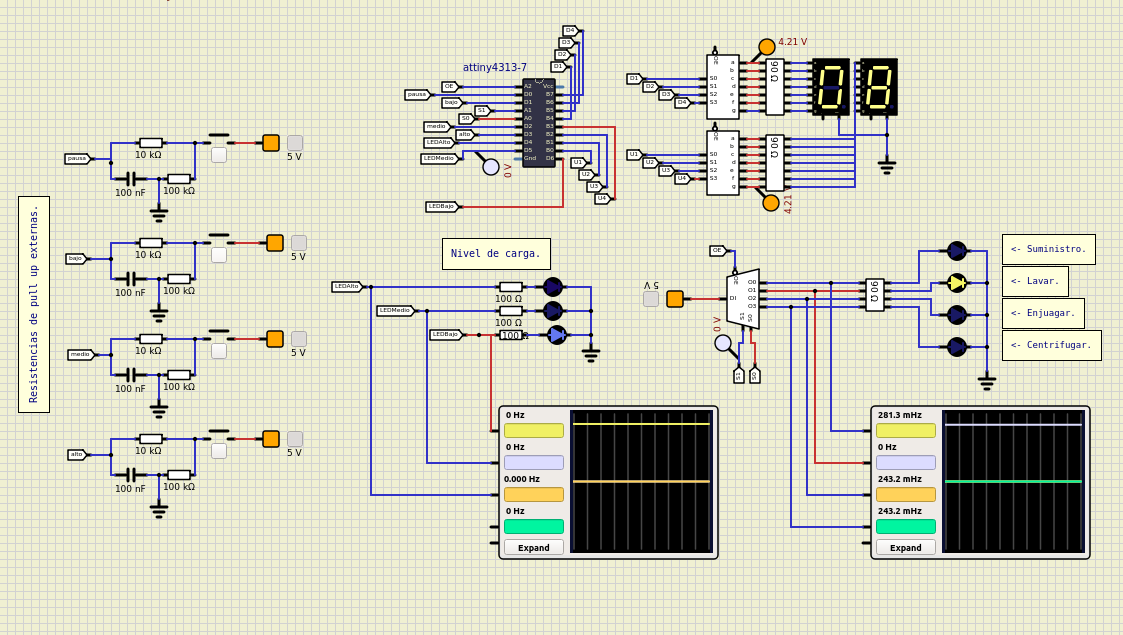
\includegraphics[width=.7\linewidth]{Imagenes/11.png}
     \caption{Carga baja lavándose.}\label{F17}
   \end{minipage}\hfill
   \begin{minipage}{0.48\textwidth}
     \centering
     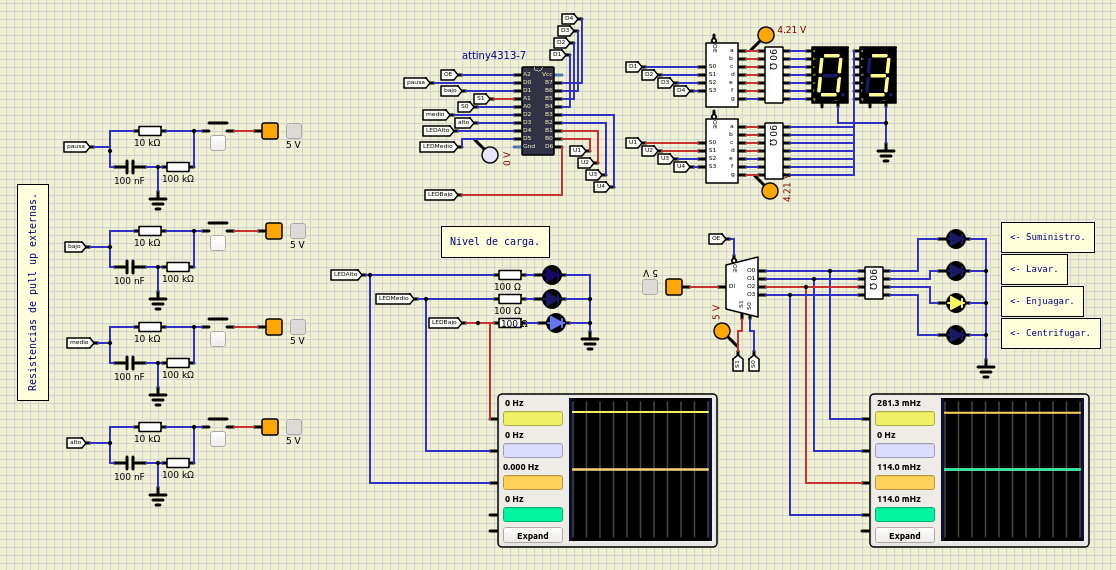
\includegraphics[width=.7\linewidth]{Imagenes/12.png}
     \caption{Carga baja lavándose parte 2. }\label{F18}
   \end{minipage}
\end{figure}
Al presionar el botón bajo, note que el fluido de corriente se va para el pin D6, y las combinaciones de los displays se envía a las etiquetas S0 y S1, que cambiarán conforme avancen los estados. También, en el osciloscopio conectado en la sección de nivel de carga, note que la señal de LEDBajo se mantiene en alto, mientras que las demás en bajo. Luego, en el siguiente osciloscopio, se muestra la cuenta regresiva del estado de suministro, la cual es de 1 segundo, de manera inmediata se tiene el estado de lavar que toma 3 segundos, para el estado de lavar, luego el siguiente estado de enjuagar que toma 2 segundos, y esto es consistente con el tiempo que le pertenece al estado de centrifugar, o sea, 3 segundos y con esto concluye el comportamiento de la carga baja. El otro detalle es que las magnitudes de las tensiones no superaron los valores máximos de los componentes electrónicos, por tanto, están seguros y no tendrán ningún daño.\par

Para cuando se presiona el botón de carga media, se obtiene el mismo comportamiento anterior, con la diferencia en los tiempos de cada estado de la lavadora. Se inicia con el estado de suministro, que debe durar 2 segundos, tanto el LED como la señal del osciloscopio se mantienen en alto y tensión eléctrica presente en el pin D5 es la adecuada para un buen funcionamiento, además, las interrupciones para que este evento sea acertado fueron ya establecidas. 
\begin{figure}[H]
        \centering
        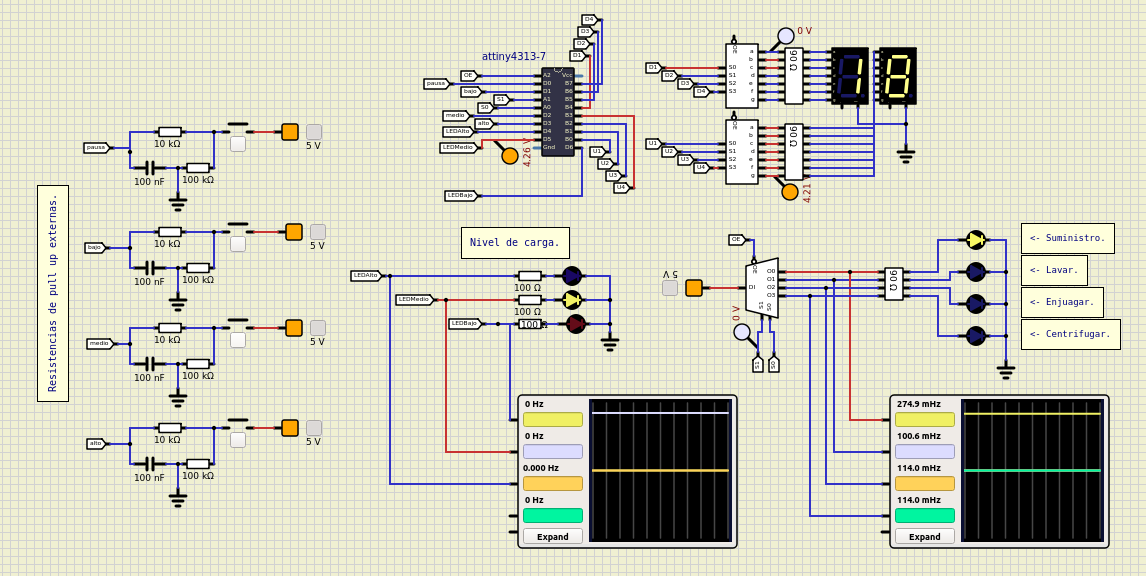
\includegraphics[width=.7\linewidth]{Imagenes/14.png}
        \caption{Estado suministro, carga media.}
        \label{fig19}
    \end{figure}
Ahora, gracias a la máquina de estados programada es posible observar el siguiente estado: lavar, 
\begin{figure}[H]
        \centering
        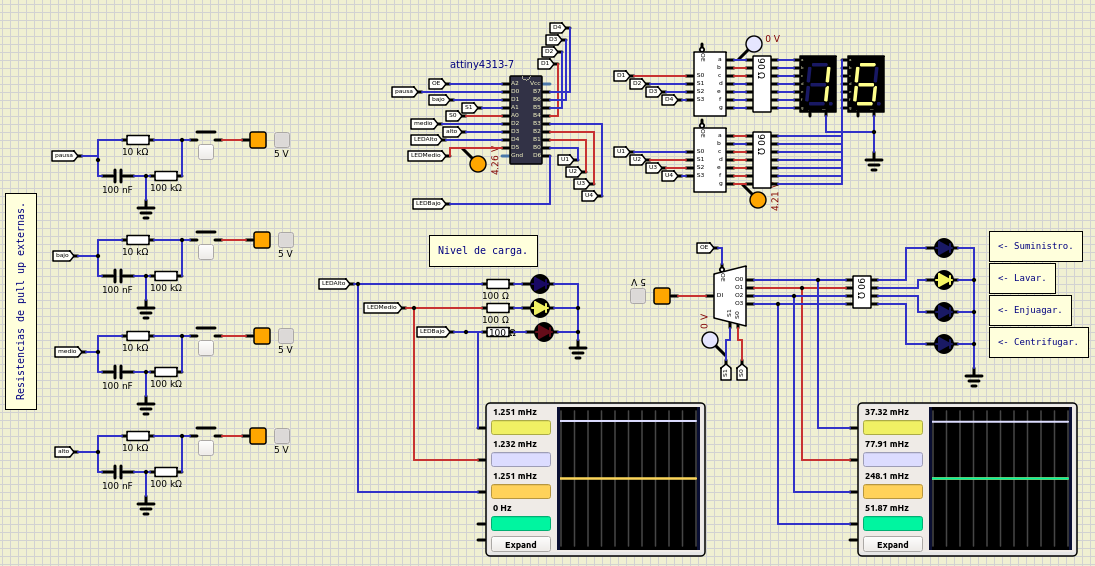
\includegraphics[width=.7\linewidth]{Imagenes/14.1.png}
        \caption{Estado lavar, carga media.}
        \label{fig20}
    \end{figure}
dicha máquina es la que decide si pasar o no a un estado al otro por medio de un intervalo de tiempo ya establecido , así para cada uno de los estados de lavado. Para la etapa de enjuague se tiene la cuenta correctamente, es decir, dura los 4 segundos y las tensiones eléctricas funcionan apropiadamente.
\begin{figure}[H]
        \centering
        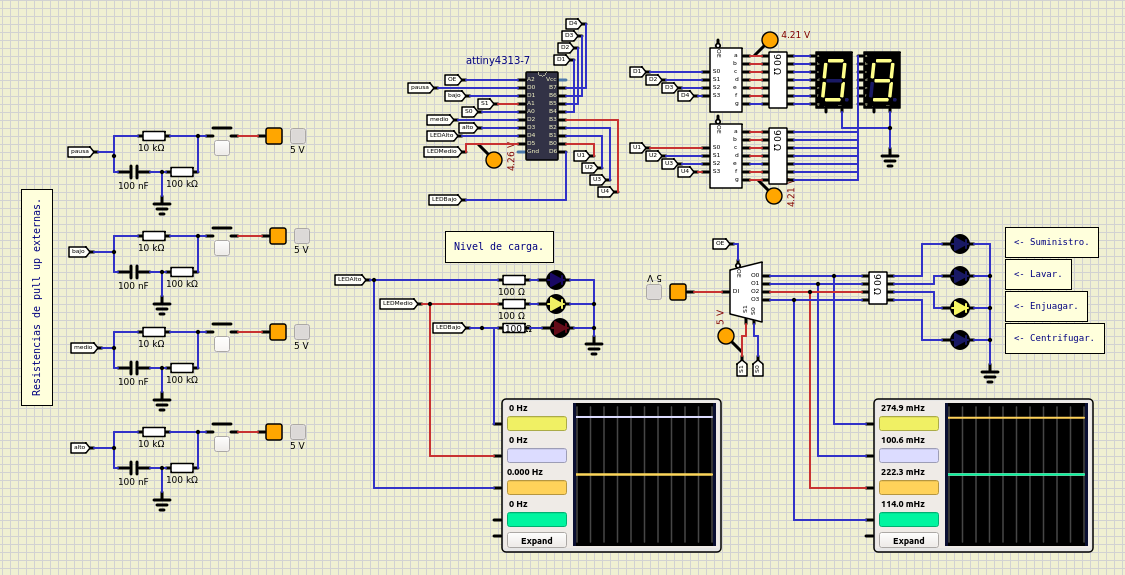
\includegraphics[width=.7\linewidth]{Imagenes/15.png}
        \caption{Estado enjuagar, carga media.}
        \label{fig21}
    \end{figure}
Por último, el manejo de la rutina por medio de \texttt{ISR(TIMER1\_COMPA\_vect)} y \texttt{ISR(TIMER0\_COMPA\_vect)} fue posible tener la actualización de los LEDs conforme avanza el tiempo, de lo contrario, los intervalos de tiempo ya establecidos no harían nada. Gracias a esto se obtiene el estado de centrifugar.
\begin{figure}[H]
        \centering
        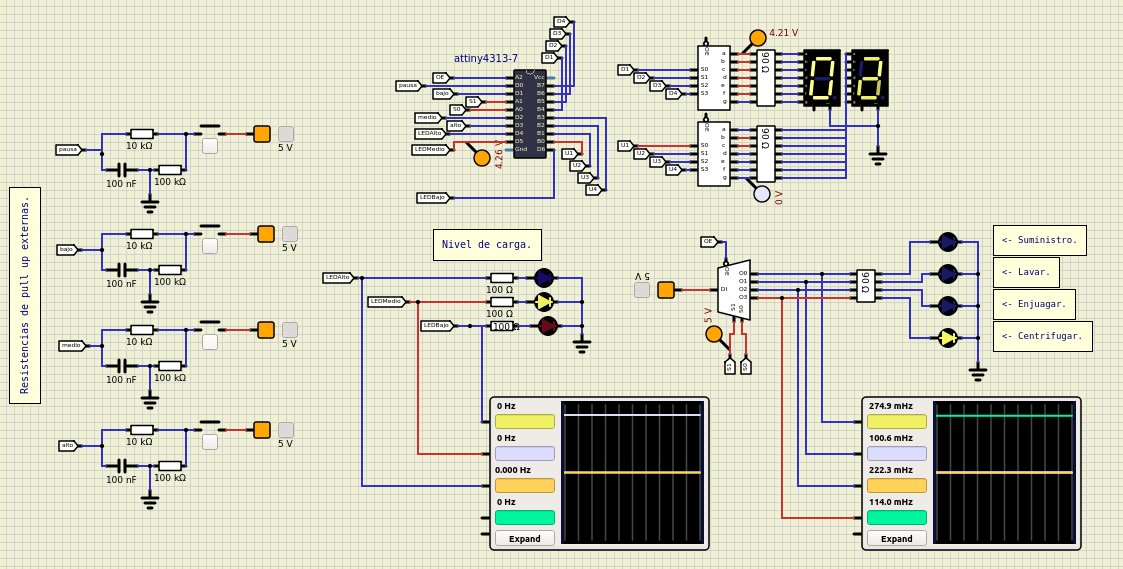
\includegraphics[width=.7\linewidth]{Imagenes/16.png}
        \caption{Estado centrifugar, carga media.}
        \label{fig22}
    \end{figure}
Finalmente, cuando se presiona el botón de carga alta, la señal de interrupción se envía correctamente, las etiquetas de los LEDs para esta carga todos están activos, las señales del osciloscopio se respetan, así como la transición de los estados. La tensión eléctrica presente en los displays es de \SI{4.21}{\volt} es la adecuada porque éstos no parpadean, esto quiere decir que nos les está llegando corriente muy alta. Por lo que se concluye que el programa es capaz de reconocer cuando se le coloca una carga alta, tal como se muestra en la siguiente transición de los estados.
\begin{itemize}
\item Estado suministro:
\begin{figure}[H]
        \centering
        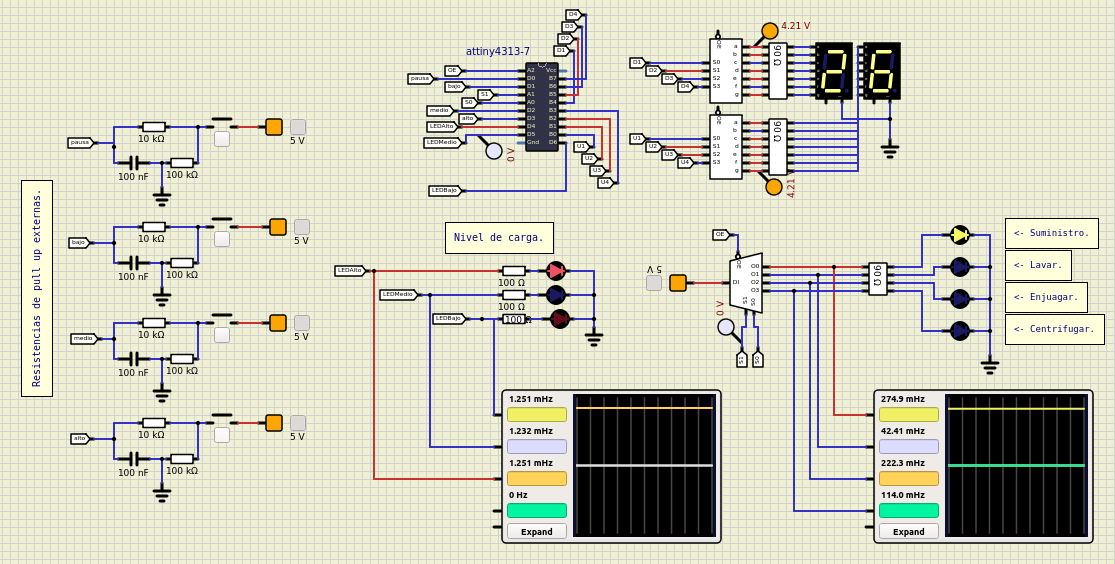
\includegraphics[width=.7\linewidth]{Imagenes/17.png}
        \caption{Estado suministro, carga alta.}
        \label{fig23}
    \end{figure}
\item Estado lavar:
\begin{figure}[H]
        \centering
        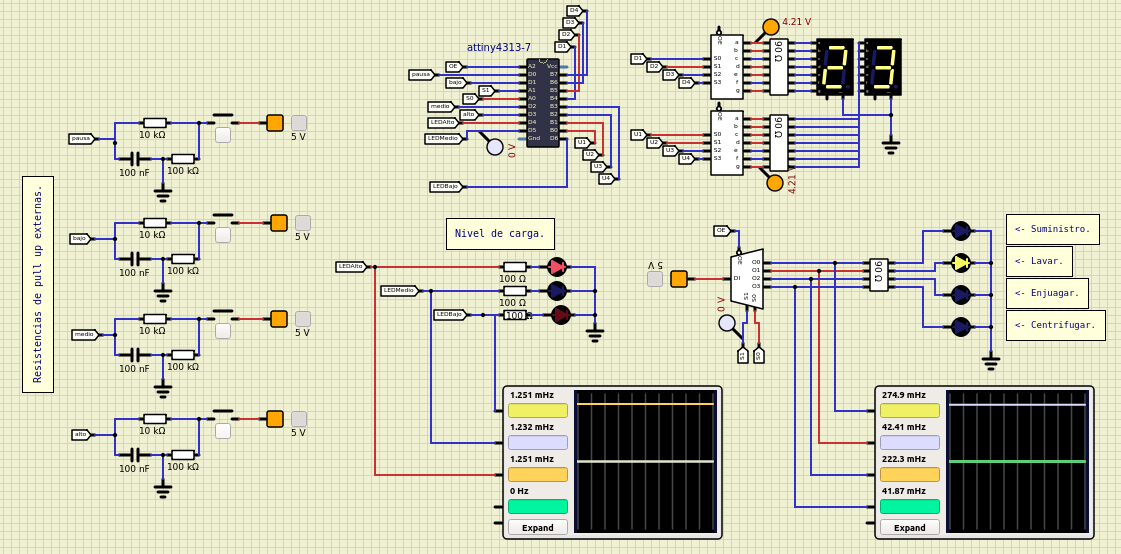
\includegraphics[width=.7\linewidth]{Imagenes/18.png}
        \caption{Estado lavar, carga alta.}
        \label{fig24}
    \end{figure}
\item Estado enjuague:
\begin{figure}[H]
        \centering
        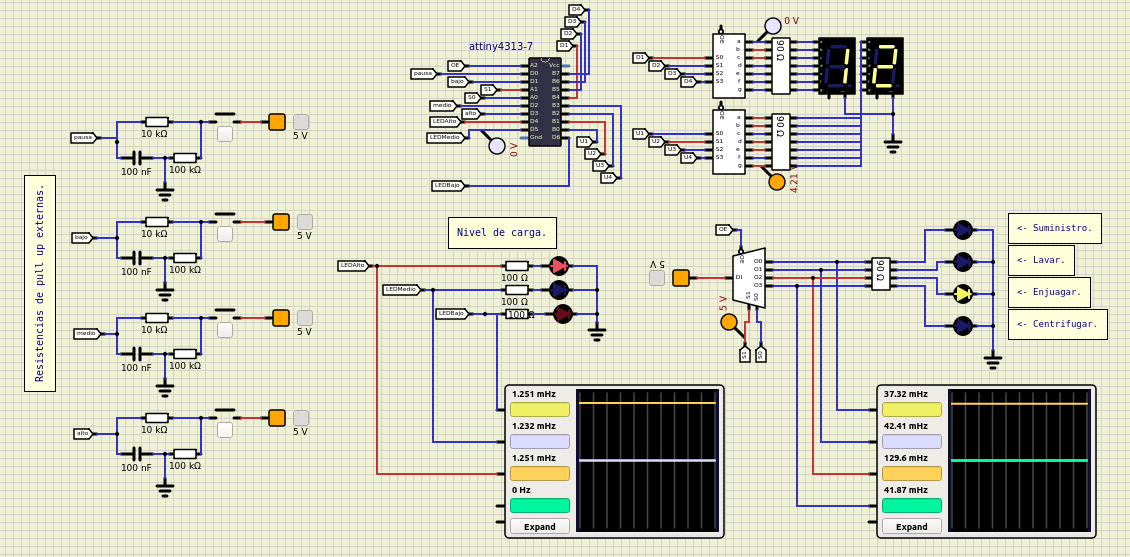
\includegraphics[width=.7\linewidth]{Imagenes/19.png}
        \caption{Estado enjuague, carga alta.}
        \label{fig25}
    \end{figure}
\item Estado centrifugar:
\begin{figure}[H]
        \centering
        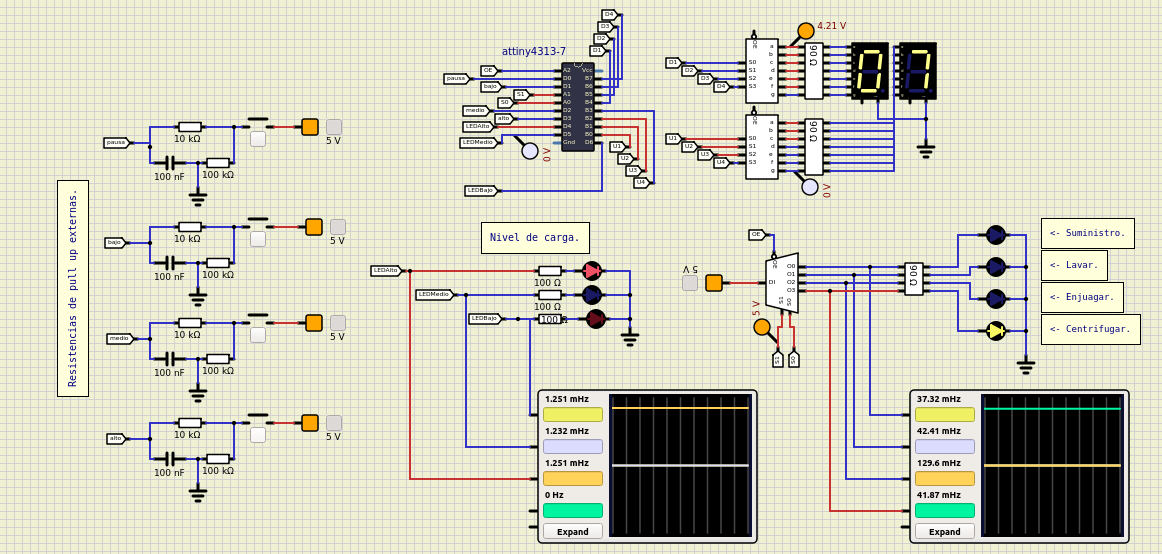
\includegraphics[width=.7\linewidth]{Imagenes/20.png}
        \caption{Estado centrifugar, carga alta.}
        \label{fig26}
    \end{figure}
\end{itemize}
En resumen, el haber configurado los temporizadores: \texttt{Timer/Counter0} y \texttt{Timer/Counter1} para hacer uso de \texttt{CTC}, los registros \texttt{TCCR04}, \texttt{WGM01} junto con un valor de comparación en las macros \texttt{OCR0A} y \texttt{OCR1A}, así como el uso de pre-escaler con sus respectivos registros, esto para reducir la señal eléctrica de alta frecuencia a una frecuencia menor por medio de una división \cite{web}, y también el uso de las interrupciones para cada timer. Esto en conjunto, con las máquinas de estado y las demás funciones permiten el buen funcionamiento de la lavadora automática.




\section{Conclusiones y recomendaciones}
Para concluir, en este trabajo fue posible entender el comportamiento de un MCU por medio del uso de interrupciones, lo que es una manera avanzada para controlar comportamientos de otros dispositivos electrónicos, por ejemplo: LEDs y displays de 7 segmentos. El haber realizado una lectura detenida de la hoja del fabricante del MCU y luego realizar pruebas excesivas para comprender el funcionamiento de cada pin fue algo muy importante para darle sentido a lo solicitado en este trabajo. La falta de literatura disponible hizo que se realizaran muchos experimentos de acuerdo a la necesidad de este laboratorio, no se escatimó el tiempo dedicado a las muchas depuraciones que se realizaron, no obstante, fueron valiosas y poder tener una simulación adecuada para esta lavadora, pues por falta de tiempo no se logró la optimización esperado en el uso de los pines, es decir, hicieron falta para poder implementar el botón de inicio y pausa, por lo que la lavadora automática está programada de tal que seleccionar la carga ésta inicia su trabajo y se detiene hasta cuando termine el tiempo asignado para cada etapa de lavado. Lo anterior se pudo haber arreglado implementando otro demultiplexor para generar las salidas de los LEDs de las cargas, ya que con las 3 salidas de los pines D4, D5 y D6 se pudo tener $2^3 = 8$ salidas o inclusive solamente trabajar con 2 salidas similar al caso de los estados, sin embargo no se implementó porque habría que cambiar el código implementado y como se mencionó anteriormente hubo una limitación de tiempo. Mucho del tiempo perdido fue debido a que se intentó hacer que los números aparecieran con solamente 5 bits en lugar de los 8 utilizados, uno de las señales de los 5 bits se invertía cada vez que se llamaba el el temporizador de los displays de esta manera solo se activaba uno en un instante dado, sin embargo, esta implementación no se logró porque el número de las decenas tomaba el de las unidades. \par
Aún así, el trabajo realizado es satisfactorio en cuanto a funcionamiento porque las interrupciones funcionaron correctamente, es decir, los LEDs responden a ellas, los temporizadores respetan los tiempos de ejecución, en ese sentido, el trabajo fue impecable. 
Como recomendaciones para este trabajo:
\begin{itemize}
\item Hacer todas las depuraciones posibles para entender el funcionamiento de lo que se está realizando.
\item Revisar las configuraciones de las interrupciones, porque es posible que se olvidé realizar alguna habilitación y esto hace que se obtenga el resultado no esperado, y el compilador tampoco se lo va a decir. En ese sentido, revisar muy bien que botones son los que se usarán para interrupciones y cuales serán simplemente salidas.
\item La siguiente página fue de mucha utilidad para el cálculo de los tiempos de los temporizadores:\\
https://eleccelerator.com/avr-timer-calculator/
\end{itemize}


\newpage 

\bibliographystyle{unsrt}
\bibliography{bibliografia.bib}
\newpage

  \section{Anexos}
 Aquí van las hojas del fabricante de los componentes usados para este laboratorio. 
\foreach \page in {1,2,3,4,5,62-68}{
  \includepdf[pages=\page]{./Documentos/ATtiny2313.pdf}
}


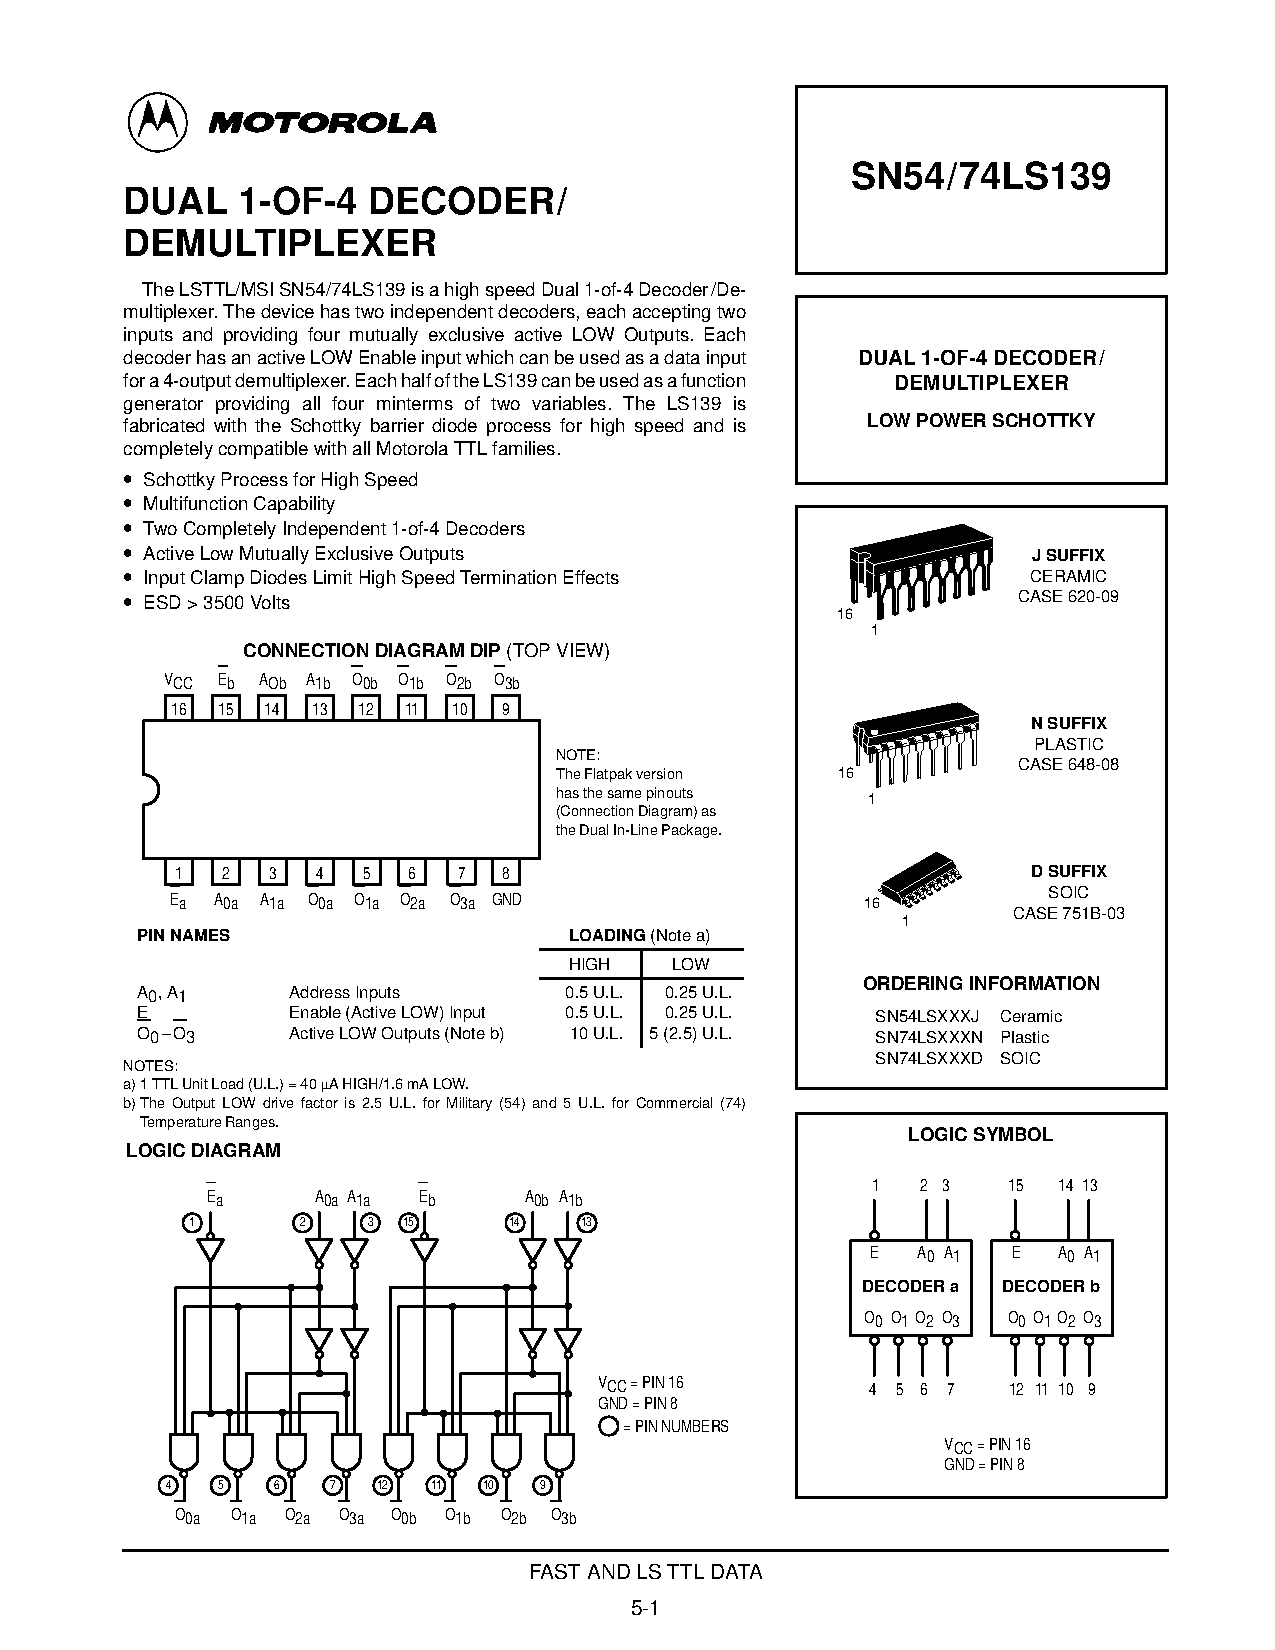
\includepdf[pages=1]{./Documentos/74LS139 Datasheet.pdf}


%\foreach \page in {1,2,3}{
%  \includepdf[pages=\page]{./Documentos/cd4511b.pdf}
%}
%\foreach \page in {1,2,3}{
%  \includepdf[pages=\page]{./Documentos/cd4511b.pdf}
%}
%\foreach \page in {2,3,4}{
%  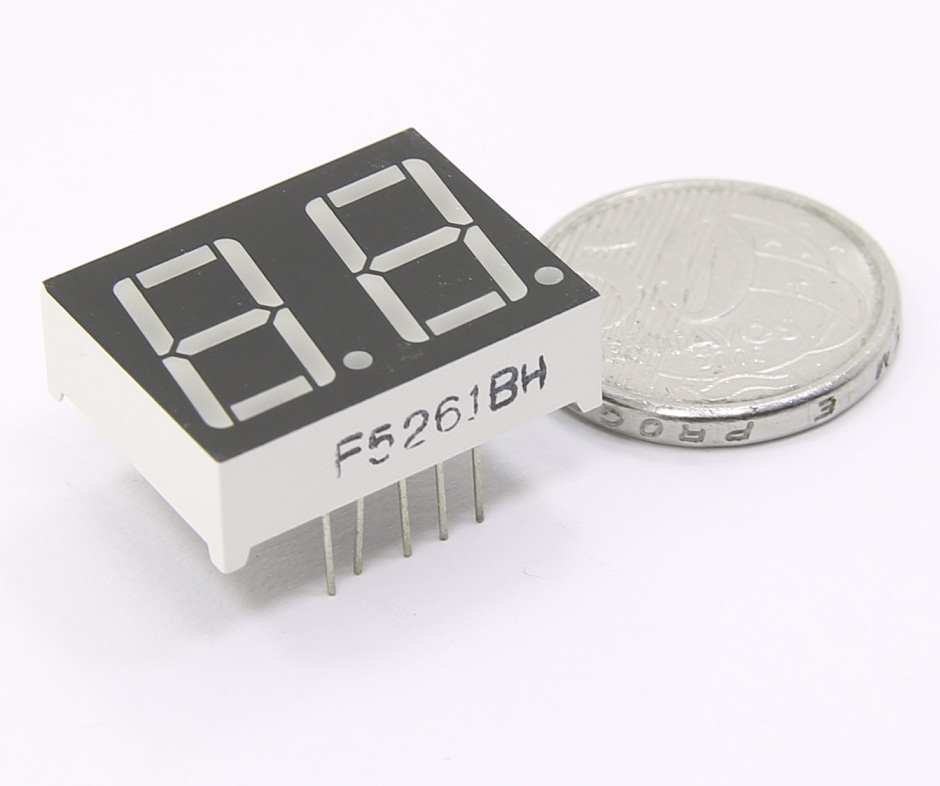
\includepdf[pages=\page]{./Documentos/display.pdf}
%}
%\includepdf[pages=1]{./Documentos/Pot.pdf}
\end{document}
 

\end{document}